\chapter{堆積與優先佇列}
\label{ch:heaps}

% 本章的圖共用的樣式與巨集（名稱都以 hp 開頭，避免和其他章衝突）
\tikzset{
    hpn/.style={circle, draw=black!65, minimum size=0.66cm, inner sep=0pt, font=\small},
    hpa/.style={hpn, draw=memStroke, thick, fill=memFill},
    hpb/.style={hpn, draw=optStroke, thick, fill=optFill},
    hpg/.style={hpn, draw=black!30, text=black!40},
    hpe/.style={hpn, draw=black!40, densely dashed},
    hpedge/.style={draw=black!55},
    hpidx/.style={font=\scriptsize, text=black!50},
    hpcn/.style={cell, minimum width=0.8cm, minimum height=0.75cm},
    hpca/.style={hpcn, draw=memStroke, thick, fill=memFill},
    hpcb/.style={hpcn, draw=optStroke, thick, fill=optFill},
    hpcg/.style={hpcn, text=black!35},
}
% \hpheap{根的座標}{最底層的寬度}{值/樣式,值/樣式,...}{節點名稱前綴}
% 依陣列順序（從 1 開始）畫一棵完整二元樹。樣式是 n、a、b、g、e 之一（e 是空的根）。
% \hpshowidxtrue 之後畫的樹，每個節點右上角會標出它在陣列裡的位置。
\newif\ifhpshowidx
\newcommand{\hpheap}[4]{%
    \foreach \hpv/\hps [count=\hpi] in {#3} {%
        \pgfmathtruncatemacro{\hplev}{floor(ln(\hpi)/ln(2) + 0.0001)}%
        \pgfmathsetmacro{\hpx}{(\hpi - 2^\hplev + 0.5) * #2 / 2^\hplev - #2 / 2}%
        \node[hp\hps] (#4\hpi) at ($(#1) + (\hpx, -0.95*\hplev)$) {\hpv};%
        \ifhpshowidx
            \node[hpidx, anchor=south west] at (#4\hpi.north east) {\hpi};%
        \fi
        \ifnum\hpi>1
            \pgfmathtruncatemacro{\hpp}{floor(\hpi/2)}%
            \draw[hpedge] (#4\hpp) -- (#4\hpi);%
        \fi
    }%
}
% \hparray{左端的座標}{值/樣式,...}：一排格子，下面標位置（從 1 開始）。
\newcommand{\hparray}[2]{%
    \foreach \hpv/\hps [count=\hpi] in {#2} {%
        \node[hpc\hps] at ($(#1) + (0.8*\hpi, 0)$) {\hpv};%
        \node[idxlbl] at ($(#1) + (0.8*\hpi, -0.6)$) {\hpi};%
    }%
}

醫院急診室的護理站旁邊有一塊白板，寫著正在等候的病人和他們的檢傷級數：1 級最緊急，
5 級最輕微。 每次有診間空出來，護理師就叫級數最小的人；級數一樣時，先到的先看。
病人隨時會來，等候中的人病情也可能變重，要往前排。 白板上的名單如果照到達順序寫，
每次叫號都要從頭看到尾；如果一直保持由急到緩排好，每來一個人又要找位置插進去，後面
的人全部往下挪。 有沒有一種寫法，讓「來一個人」和「叫一個人」都不必看過整份名單？
往下讀之前，先想一想。

這種「每次只要最大或最小的那一個」的需求叫\textbf{優先佇列}（priority queue）。 第~6~章
的佇列依進入的先後取出，優先佇列則依每個元素的\textbf{鍵}（key）大小取出。 最常用的實
作是\textbf{二元堆積}（binary heap）：把元素放在一個陣列裡，看成一棵形狀固定的二元樹，
只要求「父節點不比子節點小」，不要求整個排好。 這個較弱的要求讓插入和取出最大值都
是 $O(\lg n)$，從一堆亂數建出堆積只要 $\Theta(n)$。

本章前四節講二元堆積和它的變化：陣列存法與上浮、下沉，由下而上建堆積為什麼是線性
時間，帶索引的堆積怎麼支援 decrease-key，以及每個節點有 $d$ 個子節點的 $d$ 元堆積。
第~\ref{sec:hp-mergeable}~節講考試常見的變形：同時取最小和最大的三種結構（最小最大堆積、
deap、對稱最小最大堆積），以及可以快速合併的左傾樹和二項堆積，都以手算追蹤為主。 接著用
第~3~章的位能法，整理費氏堆積各操作的平攤成本。 章末收了幾題研究所入學考試的原題，詳解
在本章最後。

這一章用到第~7~章的樹的名詞（深度、高度、完整二元樹）和第~3~章的平攤分析；C 程式用到
《C 程式設計基礎》第~14~章的結構指標、第~15~章的遞迴和第~19~章的 \texttt{malloc}、
\texttt{realloc}，用到時先在框裡複習。 順帶一提，《C 程式設計基礎》第~19~章 19.2 節
說的 heap 是 \texttt{malloc} 配置記憶體的區域，和這一章的堆積只是同名，兩者沒有關係。

\section{二元堆積}
\label{sec:hp-binary}

\subsection{完整二元樹與陣列存法}

堆積用的是第~7~章的\textbf{完整二元樹}（complete binary tree，CLRS 第 6 章叫 nearly
complete binary tree）：除了最後一層，每一層都填滿，最後一層的節點靠左排。 第~\ref{sec:bt-array}~節說過，把完整二元樹一層一層、
每層由左到右編號 $1, 2, \ldots, n$，就能剛好填滿陣列 $A[1..n]$，不需要任何指標，父子的
位置都用算的：
\[
\proc{Parent}(i) = \lfloor i / 2 \rfloor, \qquad
\proc{Left}(i) = 2i, \qquad
\proc{Right}(i) = 2i + 1.
\]
$\proc{Left}(i) > n$ 表示 $i$ 沒有左子節點，也就是 $i$ 是葉節點；$\proc{Right}(i) > n$ 表示沒
有右子節點。

C 的陣列從 $0$ 開始。 照第~1~章的約定整段改寫，不逐個加減 $1$：位置 $i$ 的父節點是
\texttt{(i - 1) / 2}，子節點是 \texttt{2 * i + 1} 和 \texttt{2 * i + 2}。 這兩組公式是
最常寫錯的地方，寫程式時先拿 $i = 0$、$1$、$2$ 驗一次。

完整二元樹的形狀只由 $n$ 決定，這一章會一直用到下面兩個性質：

\begin{itemize}
\item \textbf{高度}是 $\lfloor \lg n \rfloor + 1$（高度數節點），位置 $i$ 的\textbf{深度}是
$\lfloor \lg i \rfloor$，見定理~\ref{thm:bt-complete-height}。
\item \textbf{葉節點}是位置 $\lfloor n/2 \rfloor + 1$ 到 $n$，共 $\lceil n/2 \rceil$ 個。 因為
$i$ 有子節點的條件是 $2i \le n$，也就是 $i \le \lfloor n/2 \rfloor$。
\end{itemize}

\subsection{堆積性質}

\begin{definition}[最大堆積、最小堆積]
\label{def:hp-heap}
存在陣列 $A[1..n]$ 的完整二元樹，如果每個 $i = 2, 3, \ldots, n$ 都滿足
$A[\lfloor i/2 \rfloor] \ge A[i]$，就叫\textbf{最大堆積}（max-heap）；如果每個 $i$ 都滿足
$A[\lfloor i/2 \rfloor] \le A[i]$，就叫\textbf{最小堆積}（min-heap）。 這個條件叫
\textbf{堆積性質}（heap property）。
\end{definition}

堆積性質只管父子之間。 沿著父節點往上走，值不會變小，所以最大堆積裡，每個節點都是它
那棵子樹的最大值，整個堆積的最大值在 $A[1]$。 兄弟之間、不同子樹之間則沒有任何規定：
堆積不是排好的陣列。 反過來，由大到小排好的陣列一定是最大堆積。

下圖是一個有 $8$ 個元素的最大堆積，右上角的小字是它在陣列裡的位置。

\begin{center}
\begin{tikzpicture}
\hpshowidxtrue
\hpheap{0,0}{6.4}{71/n,62/n,53/n,40/n,47/n,18/n,26/n,35/n}{t}
\hpshowidxfalse
\hparray{4.2,-1.4}{71/n,62/n,53/n,40/n,47/n,18/n,26/n,35/n}
\node[font=\small, anchor=west] at (4.6,-0.55) {陣列 $A[1..8]$};
\end{tikzpicture}
\diagcaption{一個最大堆積的兩種樣子。 左邊是樹，右邊是實際存的陣列。 $A[4] = 40$ 的父節
點是 $A[2] = 62$，子節點是 $A[8] = 35$；$A[5]$ 到 $A[8]$ 是葉節點。}
\label{fig:hp-heap-array}
\end{center}

\subsection{上浮與下沉}

堆積的所有操作都建立在兩個修補動作上。 假設整個陣列只有一個位置 $i$ 可能違反堆積性
質：

\begin{itemize}
\item $A[i]$ 可能比父節點大：把它和父節點交換，再看新位置和新的父節點，一路往上，直到
不比父節點大或是到了根。 這叫\textbf{上浮}（sift-up）。
\item $A[i]$ 可能比子節點小（$i$ 的兩棵子樹本身都是堆積）：把它和\textbf{較大的}子節點交
換，一路往下，直到不比任何子節點小或是到了葉節點。 這叫\textbf{下沉}（sift-down，CLRS
叫 \textsc{Max-Heapify}）。
\end{itemize}

下沉一定要和較大的子節點換。 換上來的那個數要當另一個子節點的父節點，只有較大的那個
才不會比另一邊小。

陣列 $A$ 帶一個欄位 $A.\mathit{size}$，記目前堆積裡有幾個元素；$A[A.\mathit{size}+1]$
以後的格子不屬於堆積。

\begin{pseudo}[label=alg:hp-sift]{上浮與下沉（最大堆積）}
\Procedure{Sift-Up}{$A, i$}
    \While{$i > 1$ \AND $A[\lfloor i/2 \rfloor] < A[i]$}
        \State 交換 $A[i]$ 和 $A[\lfloor i/2 \rfloor]$
        \State $i \gets \lfloor i/2 \rfloor$
    \EndWhile
\EndProcedure
\Statex
\Procedure{Sift-Down}{$A, i$}
    \While{$2i \le A.\mathit{size}$}
        \State $j \gets 2i$ \Comment{左子節點}
        \If{$j + 1 \le A.\mathit{size}$ \AND $A[j + 1] > A[j]$}
            \State $j \gets j + 1$ \Comment{右子節點比較大}
        \EndIf
        \If{$A[i] \ge A[j]$}
            \State \Return
        \EndIf
        \State 交換 $A[i]$ 和 $A[j]$
        \State $i \gets j$
    \EndWhile
\EndProcedure
\end{pseudo}

\proc{Sift-Up} 每一輪往上一層，最多 $\lfloor \lg n \rfloor$ 輪（最深的節點深度是
$\lfloor \lg n \rfloor$，也就是高度減 $1$）；\proc{Sift-Down} 每一輪往下一層，從位置 $i$
開始最多走「$i$ 的高度減 $1$」輪（$i$ 的高度是以 $i$ 為根的子樹的層數），每輪比較兩次
（第 8 行和第 10 行）。
兩者都是 $O(\lg n)$。

為什麼下沉之後整棵子樹都是堆積？ 一輪交換之前，$A[i]$ 的兩棵子樹都是堆積；換完之後
$A[i]$ 是原本三個數裡最大的，所以 $i$ 和兩個子節點之間沒問題，沒被換到的那棵子樹也沒
動過。 唯一可能出問題的是被換下去的那個數，它現在在位置 $j$，而 $j$ 的兩棵子樹仍然是
堆積，這正是下一輪的前提。 上浮的道理一樣：被換下來的父節點原本就不比它的其他子孫小，
換下來以後仍然是那棵子樹的最大值。

\subsection{插入與取出最大值}

\textbf{插入}：把新元素放到陣列最後一格，堆積多一格，形狀仍是完整二元樹；唯一可能違反
的地方是新元素和它的父節點，所以做一次上浮。

\textbf{取出最大值}：最大值在 $A[1]$。 把最後一個元素搬到 $A[1]$，堆積少一格，形狀仍是
完整二元樹；唯一可能違反的地方是新的根，它的兩棵子樹都沒動過，所以做一次下沉。

\begin{pseudo}[label=alg:hp-insert-extract, unbreakable]{插入與取出最大值}
\Procedure{Heap-Insert}{$A, x$} \Comment{假設陣列還有空間}
    \State $A.\mathit{size} \gets A.\mathit{size} + 1$
    \State $A[A.\mathit{size}] \gets x$
    \State \Call{Sift-Up}{$A, A.\mathit{size}$}
\EndProcedure
\Statex
\Function{Heap-Extract-Max}{$A$}
    \If{$A.\mathit{size} = 0$}
        \State \Error{下溢}
    \EndIf
    \State $\mathit{max} \gets A[1]$
    \State $A[1] \gets A[A.\mathit{size}]$
    \State $A.\mathit{size} \gets A.\mathit{size} - 1$
    \State \Call{Sift-Down}{$A, 1$}
    \State \Return $\mathit{max}$
\EndFunction
\end{pseudo}

兩個操作都是 $O(\lg n)$。 只看最大值不取出（\proc{Heap-Maximum}）直接回傳 $A[1]$，是
$\Theta(1)$。 最小堆積把所有的 $<$、$>$ 對調即可，之後提到「最小堆積的上浮、下沉」都是
指這個對調過的版本。

\subsection{手算追蹤}
\label{sec:hp-trace}

把 $35, 62, 18, 47, 71, 26, 53, 40$ 依序插入一個空的最大堆積，再取出兩次最大值。 下表
每一列是一個操作做完之後的陣列，「交換」是上浮或下沉交換了幾次。

\begin{center}
\begin{tabular}{lc*{8}{c}}
\toprule
操作 & 交換 & 1 & 2 & 3 & 4 & 5 & 6 & 7 & 8 \\
\midrule
插入 35 & 0 & 35 \\
插入 62 & 1 & 62 & 35 \\
插入 18 & 0 & 62 & 35 & 18 \\
插入 47 & 1 & 62 & 47 & 18 & 35 \\
插入 71 & 2 & 71 & 62 & 18 & 35 & 47 \\
插入 26 & 1 & 71 & 62 & 26 & 35 & 47 & 18 \\
插入 53 & 1 & 71 & 62 & 53 & 35 & 47 & 18 & 26 \\
插入 40 & 1 & 71 & 62 & 53 & 40 & 47 & 18 & 26 & 35 \\
\midrule
取出 71 & 2 & 62 & 47 & 53 & 40 & 35 & 18 & 26 \\
取出 62 & 1 & 53 & 47 & 26 & 40 & 35 & 18 \\
\bottomrule
\end{tabular}
\end{center}

插入 $71$ 時，它先放在 $A[5]$。 插入之前 $A[1] = 62$、$A[2] = 47$，所以 $71$ 先和
$A[2] = 47$ 交換，再和 $A[1] = 62$ 交換，共兩次；$47$ 被換到 $A[5]$，$62$ 被換到 $A[2]$。
手算時最容易出錯的是拿錯一列的陣列，每一步都要從上一列抄起。

第一次取出最大值的過程畫成樹如下：最後一個元素 $35$ 搬到根，和較大的子節點 $62$ 交換，
再和較大的子節點 $47$ 交換，到了沒有子節點的 $A[5]$ 停下。

\begin{center}
\begin{tikzpicture}
\hpheap{0,0}{4.6}{35/a,62/n,53/n,40/n,47/n,18/n,26/n}{p}
\hpheap{5.4,0}{4.6}{62/n,35/a,53/n,40/n,47/n,18/n,26/n}{q}
\hpheap{10.8,0}{4.6}{62/n,47/n,53/n,40/n,35/a,18/n,26/n}{r}
\node[font=\small] at (0,-3.0) {(a) $35$ 搬到根};
\node[font=\small] at (5.4,-3.0) {(b) 和 $62$ 交換};
\node[font=\small] at (10.8,-3.0) {(c) 和 $47$ 交換，停};
\end{tikzpicture}
\diagcaption{取出 $71$ 之後的下沉。 橘色是正在往下走的 $35$。 每一步比較它和兩個子節點，
和較大的那個交換。}
\label{fig:hp-extract}
\end{center}

\begin{examnote}
堆積的追蹤題通常要求「每插入（刪除）一個元素後畫出堆積」。 樹和陣列可以只畫一種，
但要看清楚題目要哪一種；畫樹時節點的左右位置要對，因為左右決定了陣列的順序。 兩個
子節點相等時，下沉換哪一邊會影響之後的形狀，本書一律換左邊（虛擬碼~\ref{alg:hp-sift} 第 8 行用 $>$），
CLRS 的 \textsc{Max-Heapify} 也是先看左子節點、右邊要嚴格比較大才換右邊，結果一樣。
作答時寫一句你用的規則。
\end{examnote}

\subsection{C 程式}

\begin{cbookrecap}[第~14~章 14.5 節、第~19~章 19.3 節]
\texttt{h->a} 是 \texttt{(*h).a} 的簡寫：\texttt{h} 是指向結構的指標，箭號取出它指到的
那個結構的欄位。 函式要改呼叫者的結構，就傳結構的位址進去。

\texttt{realloc(p, n)} 把 \texttt{p} 指的區塊改成 \texttt{n} 個位元組，內容保留，位址可能
換掉。 要不到記憶體時回傳 \texttt{NULL}，原本的區塊還在，所以要先用另一個指標接，確定
不是 \texttt{NULL} 才蓋回去，不能直接寫 \texttt{p = realloc(p, n)}。 \texttt{realloc}
的第一個參數是 \texttt{NULL} 時，效果和 \texttt{malloc} 一樣。
\end{cbookrecap}

下面的程式從輸入讀操作：\texttt{I x} 插入 $x$，\texttt{D} 取出最大值。 每個操作之後印
出整個陣列；取出時先在括號裡印出取出的數。 陣列滿了就用 \texttt{realloc} 把容量加倍，
第~3~章證明過這樣每次插入的平攤成本仍是 $O(1)$ 加上上浮的成本。

\begin{example}[label=ex:hp-max-heap]{c}{(max\_heap.c) 陣列實作的最大堆積}
#include <stdio.h>
#include <stdlib.h>

typedef struct {
    int *a;       // a[0..size-1] 是堆積，a[0] 是根
    int size;     // 目前有幾個元素
    int cap;      // a 的容量
} MaxHeap;

static void swap(int *x, int *y)
{
    int t = *x;
    *x = *y;
    *y = t;
}

// 位置 i 的值可能比父節點大：一路往上換。
void sift_up(MaxHeap *h, int i)
{
    while (i > 0 && h->a[(i - 1) / 2] < h->a[i]) {
        swap(&h->a[(i - 1) / 2], &h->a[i]);
        i = (i - 1) / 2;
    }
}

// 位置 i 的值可能比子節點小：和較大的子節點交換，一路往下。
void sift_down(MaxHeap *h, int i)
{
    for (;;) {
        int j = 2 * i + 1;              // 左子節點
        if (j >= h->size) {
            return;                     // i 是葉節點
        }
        if (j + 1 < h->size && h->a[j + 1] > h->a[j]) {
            j++;                        // 右子節點比較大
        }
        if (h->a[i] >= h->a[j]) {
            return;
        }
        swap(&h->a[i], &h->a[j]);
        i = j;
    }
}

int heap_insert(MaxHeap *h, int x)
{
    if (h->size == h->cap) {            // 滿了：容量加倍（第 3 章）
        int ncap = h->cap == 0 ? 4 : 2 * h->cap;
        int *na = realloc(h->a, ncap * sizeof *na);
        if (na == NULL) {
            return 0;
        }
        h->a = na;
        h->cap = ncap;
    }
    h->a[h->size] = x;
    h->size++;
    sift_up(h, h->size - 1);
    return 1;
}

// 呼叫前要確定堆積不是空的。
int heap_extract_max(MaxHeap *h)
{
    int top = h->a[0];
    h->size--;
    h->a[0] = h->a[h->size];            // 最後一個元素搬到根
    sift_down(h, 0);
    return top;
}

void print_heap(const MaxHeap *h)
{
    for (int i = 0; i < h->size; i++) {
        printf("%d%c", h->a[i], i + 1 < h->size ? ' ' : '\n');
    }
    if (h->size == 0) {
        printf("empty\n");
    }
}

int main(void)
{
    MaxHeap h = {NULL, 0, 0};
    char op;
    while (scanf(" %c", &op) == 1) {
        if (op == 'I') {
            int x;
            if (scanf("%d", &x) != 1 || !heap_insert(&h, x)) {
                break;
            }
        } else if (op == 'D') {
            if (h.size == 0) {
                printf("underflow\n");
                continue;
            }
            printf("(%d) ", heap_extract_max(&h));
        } else {
            break;
        }
        print_heap(&h);
    }
    free(h.a);
    return 0;
}
\end{example}
\iosample{I 35 \\ I 62 \\ I 18 \\ I 47 \\ I 71 \\ I 26 \\ I 53 \\ I 40 \\ D \\ D}{35 \\ 62 35 \\ 62 35 18 \\ 62 47 18 35 \\ 71 62 18 35 47 \\ 71 62 26 35 47 18 \\ 71 62 53 35 47 18 26 \\ 71 62 53 40 47 18 26 35 \\ (71) 62 47 53 40 35 18 26 \\ (62) 53 47 26 40 35 18}

輸出的每一列和上一小節的表一樣。 \texttt{heap\_extract\_max} 在只剩一個元素時也對：
\texttt{size} 變成 $0$，\texttt{a[0] = a[0]}，\texttt{sift\_down} 發現 \texttt{j >= size}
立刻返回。

\section{由下而上建堆積}
\label{sec:hp-build}

手上已經有 $n$ 個數，要把它們變成堆積。 最直接的做法是一個一個插入，每次 $O(\lg n)$，
共 $O(n \lg n)$。 這個上界是緊的：輸入由小到大時，每個新來的數都比堆積裡所有的數大，
要一路浮到根，第 $i$ 個數交換 $\lfloor \lg i \rfloor$ 次，總共
$\sum_{i=1}^{n} \lfloor \lg i \rfloor = \Theta(n \lg n)$ 次（觀念題第~\ref{hp-q-sum}~題）。

另一種做法是把 $n$ 個數直接放進 $A[1..n]$，再由下往上修補。 葉節點自己就是只有一個節點
的堆積，不用修；從最後一個有子節點的位置 $\lfloor n/2 \rfloor$ 開始，倒著對每個位置做
下沉。 輪到位置 $i$ 時，比它大的位置都已經修好了，所以 $i$ 的兩棵子樹都是堆積，正好
符合下沉的前提。

\begin{pseudo}[label=alg:hp-build]{由下而上建最大堆積}
\Procedure{Build-Max-Heap}{$A, n$}
    \State $A.\mathit{size} \gets n$
    \For{$i \gets \lfloor n/2 \rfloor$ \DownTo $1$}
        \State \Call{Sift-Down}{$A, i$}
    \EndFor
\EndProcedure
\end{pseudo}

\textbf{正確性}用迴圈不變量（第~\ref{sec:ana-invariant}~節）：第 3 行的迴圈每一輪開始時，位置
$i + 1, i + 2, \ldots, n$ 的每一個節點都是一個最大堆積的根。 初始時 $i = \lfloor n/2
\rfloor$，後面的位置都是葉節點，成立。 維持的論證就是上一段的「兩棵子樹都是堆積」。 結
束時 $i = 0$，代進去就是位置 $1$ 是最大堆積的根，也就是整個陣列是最大堆積。 （觀念題
第~\ref{hp-q-build}~題要你把三步完整寫出來。）

\subsection{手算追蹤}

用 $A = \langle 14, 37, 52, 9, 61, 28, 45, 70, 23, 66 \rangle$，$n = 10$，$i$ 從 $5$ 做到
$1$。 每一列是那一次 \proc{Sift-Down} 做完之後的陣列。

\begin{center}
\begin{tabular}{lc*{10}{c}}
\toprule
& 交換 & 1 & 2 & 3 & 4 & 5 & 6 & 7 & 8 & 9 & 10 \\
\midrule
開始 & & 14 & 37 & 52 & 9 & 61 & 28 & 45 & 70 & 23 & 66 \\
$i = 5$ & 1 & 14 & 37 & 52 & 9 & 66 & 28 & 45 & 70 & 23 & 61 \\
$i = 4$ & 1 & 14 & 37 & 52 & 70 & 66 & 28 & 45 & 9 & 23 & 61 \\
$i = 3$ & 0 & 14 & 37 & 52 & 70 & 66 & 28 & 45 & 9 & 23 & 61 \\
$i = 2$ & 1 & 14 & 70 & 52 & 37 & 66 & 28 & 45 & 9 & 23 & 61 \\
$i = 1$ & 3 & 70 & 66 & 52 & 37 & 61 & 28 & 45 & 9 & 23 & 14 \\
\bottomrule
\end{tabular}
\end{center}

$i = 5$ 只有左子節點 $A[10] = 66$；$i = 3$ 的 $52$ 已經比 $28$、$45$ 大，不用動；
$i = 1$ 的 $14$ 一路換到葉節點：先和 $70$ 換，再和 $A[4]$、$A[5]$ 中較大的 $66$ 換，最後和
$A[10] = 61$ 換。 下圖左邊是開始時的樹，右邊是建好的堆積。

\begin{center}
\begin{tikzpicture}
\hpheap{0,0}{6.0}{14/a,37/n,52/n,9/n,61/n,28/n,45/n,70/n,23/n,66/n}{s}
\hpheap{7.4,0}{6.0}{70/n,66/n,52/n,37/n,61/n,28/n,45/n,9/n,23/n,14/a}{e}
\node[font=\small] at (0,-3.6) {開始};
\node[font=\small] at (7.4,-3.6) {建好之後};
\end{tikzpicture}
\diagcaption{由下而上建堆積。 原本在根的 $14$（橘色）最後落到葉節點。}
\label{fig:hp-build}
\end{center}

同一組數如果一個一個插入，得到的是 $\langle 70, 66, 45, 52, 61, 28, 37, 9, 23, 14
\rangle$，交換 $10$ 次；由下而上建只交換 $6$ 次，結果也不一樣。 兩個都是合法的最大堆
積，考題問哪一種方法，就要照那一種做。

\begin{examnote}
題目說「建立堆積」（build a heap）而沒有指定方法時，先看題目有沒有「依序插入」之類的
字。 有就逐一插入；沒有的話，通常指的是由下而上的方法，CLRS 6.3 節的
\textsc{Build-Max-Heap} 就是這一種。 作答時先寫明你用哪一種，再寫追蹤。 由下而上的方法要從 $\lfloor n/2 \rfloor$ 開始倒著做，從 $1$ 往下做是錯的。
\end{examnote}

\subsection{為什麼是 $O(n)$}

令 $h(x)$ 是節點 $x$ 的高度，也就是以 $x$ 為根的子樹的層數，葉節點的高度是 $1$。 從 $x$
往下走到最遠的葉節點要 $h(x) - 1$ 步，所以對位置 $i$ 做 \proc{Sift-Down}，交換次數不超過
$h(i) - 1$，比較次數不超過 $2(h(i) - 1) + 2$。 所以只要證明「所有節點的 $h(x) - 1$ 加
起來是 $O(n)$」。 直覺是：一半的節點是葉節點，高度 $1$，一步都不用走；四分之一高度 $2$，
最多走一步；八分之一高度 $3$，最多走兩步……高度大的節點很少。

\begin{theorem}
\label{thm:hp-build}
有 $n$ 個節點的完整二元樹，$\sum_x \bigl(h(x) - 1\bigr) < 2n$，加總跑過所有節點。 因此
\proc{Build-Max-Heap} 的交換次數小於 $2n$，執行時間是 $\Theta(n)$。
\end{theorem}

\begin{proof}
先算\textbf{滿二元樹}（第~7~章的 perfect binary tree，每一層都填滿）。 設高度是
$k \ge 1$，共 $N = 2^k - 1$ 個節點，深度 $d$ 的節點高度是 $k - d$。 換一個方向數：對每個
$\ell = 2, 3, \ldots, k$，數「高度至少是 $\ell$」的節點有幾個，再把這些個數加起來，每個
高度 $h$ 的節點剛好被數了 $h - 1$ 次（$\ell = 2, \ldots, h$ 各一次）。 高度至少 $\ell$ 的
節點就是深度不超過 $k - \ell$ 的節點，也就是最上面 $k - \ell + 1$ 層，有
$2^{k - \ell + 1} - 1$ 個。 所以
\[
\sum_{x} \bigl(h(x) - 1\bigr)
= \sum_{\ell=2}^{k} \left(2^{k - \ell + 1} - 1\right)
= (2^k - 2) - (k - 1)
= N - k.
\]
一般的 $n$，令 $k = \lfloor \lg n \rfloor + 1$，這是這棵完整二元樹的高度。 它的節點是高度
$k$ 的滿二元樹的位置 $1..n$，每個節點的子樹只會比滿二元樹裡少，高度不會比較大；而且每一
項 $h(x) - 1$ 都不是負的，少掉的節點只會讓總和變小。 所以總和不超過
$2^k - 1 - k < 2^k = 2^{\lfloor \lg n \rfloor + 1} \le 2n$。

交換次數不超過這個總和，所以小於 $2n$；只有 $\lfloor n/2 \rfloor$ 個非葉節點要下沉，比
較次數不超過 $2\sum_x (h(x) - 1) + 2\lfloor n/2 \rfloor < 5n$。 另一方面每個元素至少要看
一次，所以是 $\Theta(n)$。
\end{proof}

其實 $\sum_x (h(x) - 1)$ 恰好是 $n - b(n)$，$b(n)$ 是 $n$ 的二進位表示中 $1$ 的個數（這裡
不證）；換成高度和就是 $2n - b(n)$。 用邊數算高度時每個節點的高度都少 $1$，同一件事
會寫成「高度和是 $n - b(n)$」。 要注意這個論證和「一共 $\lfloor n/2 \rfloor$ 次下沉、每次
$O(\lg n)$，所以 $O(n \lg n)$」並不矛盾：那個估法給的是對的上界，只是不夠緊，因為大部
分的下沉都從接近葉節點的地方開始。

把上浮和下沉寫成 C 實際數一下：輸入由小到大時，由下而上的方法在 $n = 10^6$ 只交換 $999{,}988$ 次，比
$n - b(n) = 999{,}993$ 還少一點；逐一插入則交換了大約 $1.8 \times 10^7$ 次，接近
$n \lg n - 2n$，是前者的 $18$ 倍。

\subsection{堆積排序}

建好最大堆積以後，把根（最大值）和最後一格交換，堆積縮小一格，再對根做一次下沉；重
複 $n - 1$ 次，陣列就由小到大排好了。 這就是\textbf{堆積排序}（heapsort）：原地排序，
最壞情況 $O(n \lg n)$。 它的比較次數、不穩定的原因，以及和其他排序的比較放在第~\ref{sec:so-heap}~節。

\section{優先佇列與帶索引的堆積}
\label{sec:hp-pq}

\textbf{最小優先佇列}（min-priority queue）是一個抽象資料型態（第~6~章），維護一群各自帶
有鍵的元素，支援下面的操作：

\begin{itemize}
\item \proc{Insert}$(Q, x, k)$：加入元素 $x$，鍵是 $k$。
\item \proc{Minimum}$(Q)$：回傳鍵最小的元素，不取出。
\item \proc{Extract-Min}$(Q)$：取出並回傳鍵最小的元素。
\item \proc{Decrease-Key}$(Q, x, k)$：把元素 $x$ 的鍵改成比較小的 $k$。
\item \proc{Delete}$(Q, x)$：把元素 $x$ 從佇列中拿掉。
\end{itemize}

最大優先佇列把「最小」換成「最大」，\proc{Decrease-Key} 換成 \proc{Increase-Key}。 第~25~章
的 Dijkstra 演算法和第~24~章的 Prim 演算法都用最小優先佇列，而且大量使用
\proc{Decrease-Key}，所以這一節用最小堆積來寫。

幾種實作的成本比較如下（$n$ 是佇列裡的元素個數；\proc{Decrease-Key} 假設已經知道 $x$
存在哪裡）。

\begin{center}
\begin{tabular}{lcccc}
\toprule
實作 & \proc{Insert} & \proc{Minimum} & \proc{Extract-Min} & \proc{Decrease-Key} \\
\midrule
未排序的陣列 & $\Theta(1)$ & $\Theta(n)$ & $\Theta(n)$ & $\Theta(1)$ \\
由大到小排好的陣列 & $\Theta(n)$ & $\Theta(1)$ & $\Theta(1)$ & $\Theta(n)$ \\
排好的鏈結串列 & $\Theta(n)$ & $\Theta(1)$ & $\Theta(1)$ & $\Theta(n)$ \\
二元堆積 & $O(\lg n)$ & $\Theta(1)$ & $O(\lg n)$ & $O(\lg n)$ \\
\bottomrule
\end{tabular}
\end{center}

排好的陣列由大到小放，最小值在最後一格，取出時不用挪動其他元素。 前三種總有一個操作
要 $\Theta(n)$；堆積把每個操作都壓到 $O(\lg n)$，做 $n$ 次插入、$n$ 次取出的總成本從
$\Theta(n^2)$ 降到 $O(n \lg n)$。

\subsection{decrease-key 要先知道元素在哪裡}

堆積不支援搜尋：在最小堆積裡找鍵 $k$，只能跳過根比 $k$ 大的子樹，其他的都得往下看，
最壞要看 $\Theta(n)$ 格（例如 $k$ 比所有的鍵都大）。 所以
\proc{Decrease-Key}$(Q, x, k)$ 的 $x$ 不能只是一個鍵，必須能直接找到它在陣列的位置。 常
見的做法是給每個元素一個編號 $v = 1, 2, \ldots, m$（例如圖的點、病人的掛號序號），陣列
$H.A$ 裡存的是編號，另外開兩個以編號為索引的陣列：

\begin{itemize}
\item $H.\mathit{key}[v]$：元素 $v$ 目前的鍵。
\item $H.\mathit{pos}[v]$：元素 $v$ 目前在 $H.A$ 的哪一格；不在堆積裡時是 $0$。
\end{itemize}

這叫\textbf{帶索引的堆積}（indexed heap）。 每次交換 $H.A$ 的兩格，兩個元素的
$\mathit{pos}$ 都要跟著改，所以把交換寫成一個程序。 鍵變小時，元素只可能比父節點小，
做一次上浮；刪除任意一個元素時，用最後一個元素補進它的位置，補進來的數可能比新的父節
點小，也可能比子節點大，兩個方向都要試。

\begin{pseudo}[label=alg:hp-indexed]{帶索引的最小堆積}
\Procedure{Exchange}{$H, i, j$}
    \State 交換 $H.A[i]$ 和 $H.A[j]$
    \State $H.\mathit{pos}[H.A[i]] \gets i$
    \State $H.\mathit{pos}[H.A[j]] \gets j$
\EndProcedure
\Statex
\Procedure{Decrease-Key}{$H, v, k$}
    \If{$k > H.\mathit{key}[v]$}
        \State \Error{新的鍵比原來大}
    \EndIf
    \State $H.\mathit{key}[v] \gets k$
    \State $i \gets H.\mathit{pos}[v]$
    \While{$i > 1$ \AND $H.\mathit{key}[H.A[\lfloor i/2 \rfloor]] > H.\mathit{key}[H.A[i]]$}
        \State \Call{Exchange}{$H, i, \lfloor i/2 \rfloor$}
        \State $i \gets \lfloor i/2 \rfloor$
    \EndWhile
\EndProcedure
\Statex
\Procedure{Heap-Delete}{$H, v$}
    \State $i \gets H.\mathit{pos}[v]$
    \State \Call{Exchange}{$H, i, H.\mathit{size}$}
    \State $H.\mathit{size} \gets H.\mathit{size} - 1$
    \State $H.\mathit{pos}[v] \gets 0$
    \If{$i \le H.\mathit{size}$}
        \State \Call{Min-Sift-Up}{$H, i$}
        \State \Call{Min-Sift-Down}{$H, i$}
    \EndIf
\EndProcedure
\end{pseudo}

\proc{Min-Sift-Up}、\proc{Min-Sift-Down} 是虛擬碼~\ref{alg:hp-sift} 把比較反過來、比較的
對象改成 $H.\mathit{key}[H.A[\cdot]]$、交換改成 \proc{Exchange} 的版本。 第 19、20 行兩
個都呼叫，但最多只有一個會真的動：補進來的數如果比父節點小，往上浮，浮上去的路徑上原
本的數都比它大，不會再需要下沉；反之亦然。 \proc{Extract-Min} 就是
\proc{Heap-Delete}$(H, H.A[1])$。 所有操作都是 $O(\lg n)$，多花的空間是兩個長度 $m$ 的
陣列。

有些實作不做 \proc{Decrease-Key}，鍵變小時直接再插入一份新的，舊的那份留在堆積裡，取出
時發現是過期的就丟掉。 這樣寫比較短，代價是堆積裡最多可能有和操作次數一樣多的元素。
寫 Dijkstra 演算法（第~25~章）時兩種都常見。

\subsection{例子：急診室的候診名單}

回到章首的急診室。 病人依到達順序編號 $1, 2, 3, \ldots$，鍵是（級數，編號）這一對：級
數小的優先，同級時編號小（先到）的優先。 只用級數當鍵是不夠的，堆積不會保持相同鍵的
先後順序（下沉時同一層的元素會被換來換去），所以把到達順序也放進鍵裡。

下面的程式處理一個晚上的紀錄。 \texttt{A} 是新病人到達，\texttt{T} 是叫號看診，
\texttt{U 3 1} 是 $3$ 號病人病情變化、改成 $1$ 級，\texttt{L 2} 是 $2$ 號病人沒等到就離
開。 看診和離開都是把一個病人從堆積拿掉，程式用同一個函式 \texttt{er\_remove}，也就是
虛擬碼的 \proc{Heap-Delete}。 每個操作之後印出堆積陣列，\texttt{6(2)} 表示 $6$ 號病人、
$2$ 級。

\begin{example}[label=ex:hp-er-queue]{c}{(er\_queue.c) 用帶索引的最小堆積管理候診名單}
#include <stdio.h>
#include <stdlib.h>

// 帶索引的最小堆積。病人編號 1, 2, 3, ... 依到達順序給。
// 比較的鍵是 (級數, 編號)：級數小的先看，同級的先到先看。
typedef struct {
    int *heap;    // heap[0..size-1]：放病人編號
    int *pos;     // pos[v]：病人 v 在 heap 的哪一格
    int *level;   // level[v]：病人 v 的檢傷級數（1 最緊急）
    int size;
} ERQueue;

// 病人 u 是否應該排在 v 前面
static int before(const ERQueue *q, int u, int v)
{
    return q->level[u] < q->level[v] ||
           (q->level[u] == q->level[v] && u < v);
}

// 交換 heap[i]、heap[j]，兩人的 pos 也要跟著改
static void swap_at(ERQueue *q, int i, int j)
{
    int u = q->heap[i], v = q->heap[j];
    q->heap[i] = v;
    q->heap[j] = u;
    q->pos[v] = i;
    q->pos[u] = j;
}

static void sift_up(ERQueue *q, int i)
{
    while (i > 0 && before(q, q->heap[i], q->heap[(i - 1) / 2])) {
        swap_at(q, i, (i - 1) / 2);
        i = (i - 1) / 2;
    }
}

static void sift_down(ERQueue *q, int i)
{
    for (;;) {
        int j = 2 * i + 1;
        if (j >= q->size) {
            return;
        }
        if (j + 1 < q->size &&
            before(q, q->heap[j + 1], q->heap[j])) {
            j++;
        }
        if (!before(q, q->heap[j], q->heap[i])) {
            return;
        }
        swap_at(q, i, j);
        i = j;
    }
}

void er_arrive(ERQueue *q, int v, int lv)
{
    q->level[v] = lv;
    q->heap[q->size] = v;
    q->pos[v] = q->size;
    q->size++;
    sift_up(q, q->size - 1);
}

// 看診或離開：把病人 v 拿掉，最後一個補進他的位置，再往上或往下調整。
void er_remove(ERQueue *q, int v)
{
    int i = q->pos[v];
    q->size--;
    if (i != q->size) {
        swap_at(q, i, q->size);
        sift_up(q, i);               // 兩個方向最多只有一個會動
        sift_down(q, i);
    }
}

void er_upgrade(ERQueue *q, int v, int lv)   // decrease-key
{
    q->level[v] = lv;
    sift_up(q, q->pos[v]);
}

int main(void)
{
    // 一個晚上的紀錄。A x：新病人到達，x 級；T：叫號看診；
    // U x y：x 號病人改成 y 級；L x：x 號病人離開。
    struct { char op; int x, y; } ops[] = {
        {'A', 4, 0}, {'A', 4, 0}, {'A', 5, 0}, {'A', 3, 0},
        {'A', 4, 0}, {'A', 2, 0}, {'A', 3, 0}, {'L', 2, 0},
        {'U', 3, 1}, {'A', 3, 0}, {'T', 0, 0}, {'T', 0, 0}};
    int m = sizeof ops / sizeof ops[0];      // 病人最多 m 個
    size_t sz = (m + 1) * sizeof(int);       // 編號從 1 用到 m
    ERQueue q = {malloc(sz), malloc(sz), malloc(sz), 0};
    if (q.heap == NULL || q.pos == NULL || q.level == NULL) {
        free(q.heap);
        free(q.pos);
        free(q.level);
        return 1;
    }
    int next = 1;                            // 下一個病人的編號
    for (int k = 0; k < m; k++) {
        int x = ops[k].x, y = ops[k].y;
        if (ops[k].op == 'A') {
            er_arrive(&q, next, x);
            printf("arrive %d(%d):", next, x);
            next++;
        } else if (ops[k].op == 'T') {       // 看診時一定有人
            int v = q.heap[0];
            er_remove(&q, v);
            printf("treat %d(%d):", v, q.level[v]);
        } else if (ops[k].op == 'U') {
            er_upgrade(&q, x, y);
            printf("upgrade %d(%d):", x, y);
        } else {
            er_remove(&q, x);
            printf("leave %d:", x);
        }
        for (int i = 0; i < q.size; i++) {
            printf(" %d(%d)", q.heap[i], q.level[q.heap[i]]);
        }
        printf("\n");
    }
    free(q.heap);
    free(q.pos);
    free(q.level);
    return 0;
}
\end{example}
\iosample{}{arrive 1(4): 1(4) \\ arrive 2(4): 1(4) 2(4) \\ arrive 3(5): 1(4) 2(4) 3(5) \\ arrive 4(3): 4(3) 1(4) 3(5) 2(4) \\ arrive 5(4): 4(3) 1(4) 3(5) 2(4) 5(4) \\ arrive 6(2): 6(2) 1(4) 4(3) 2(4) 5(4) 3(5) \\ arrive 7(3): 6(2) 1(4) 4(3) 2(4) 5(4) 3(5) 7(3) \\ leave 2: 6(2) 7(3) 4(3) 1(4) 5(4) 3(5) \\ upgrade 3(1): 3(1) 7(3) 6(2) 1(4) 5(4) 4(3) \\ arrive 8(3): 3(1) 7(3) 6(2) 1(4) 5(4) 4(3) 8(3) \\ treat 3(1): 6(2) 7(3) 4(3) 1(4) 5(4) 8(3) \\ treat 6(2): 4(3) 7(3) 8(3) 1(4) 5(4)}

\subsection{手算追蹤}

上面的輸出整理成考卷的寫法，一個操作一列，記陣列的內容（位置從 $1$ 開始）。

\begin{center}
\begin{tabular}{l*{7}{c}}
\toprule
操作 & 1 & 2 & 3 & 4 & 5 & 6 & 7 \\
\midrule
到達 1(4)、2(4)、3(5) & 1(4) & 2(4) & 3(5) \\
到達 4(3) & 4(3) & 1(4) & 3(5) & 2(4) \\
到達 5(4) & 4(3) & 1(4) & 3(5) & 2(4) & 5(4) \\
到達 6(2) & 6(2) & 1(4) & 4(3) & 2(4) & 5(4) & 3(5) \\
到達 7(3) & 6(2) & 1(4) & 4(3) & 2(4) & 5(4) & 3(5) & 7(3) \\
離開 2 & 6(2) & 7(3) & 4(3) & 1(4) & 5(4) & 3(5) \\
3 號改成 1 級 & 3(1) & 7(3) & 6(2) & 1(4) & 5(4) & 4(3) \\
到達 8(3) & 3(1) & 7(3) & 6(2) & 1(4) & 5(4) & 4(3) & 8(3) \\
看診 3 & 6(2) & 7(3) & 4(3) & 1(4) & 5(4) & 8(3) \\
看診 6 & 4(3) & 7(3) & 8(3) & 1(4) & 5(4) \\
\bottomrule
\end{tabular}
\end{center}

幾個值得看的步驟：

\begin{itemize}
\item \textbf{到達 6(2)}：放在第 6 格，父節點第 3 格是 3(5)，交換；到了第 3 格，父節點
4(3) 也比較後面，再交換，6 號一路到根。
\item \textbf{離開 2}：2 號在第 4 格。 最後一格的 7(3) 補進第 4 格，它比父節點 1(4) 優
先，所以要\textbf{上浮}，和 1(4) 交換。 只寫下沉的程式在這裡會出錯。
\item \textbf{3 號改成 1 級}：3 號在第 6 格，鍵變小以後上浮兩次到根，這就是
\proc{Decrease-Key}。 程式用 \texttt{pos[3]} 直接找到第 6 格，不用搜尋。
\item \textbf{看診 3}：最後一格的 8(3) 搬到根，兩個子節點 7(3)、6(2) 中 6(2) 優先，交換；
到了第 3 格，唯一的子節點 4(3) 和它同級但編號較小，所以再交換一次。
\end{itemize}

\subsection{其他常見用法}

\begin{itemize}
\item \textbf{合併 $k$ 個排好的數列}：最小堆積裡放每個數列目前的第一個數，每次取出最小
的輸出，再把它所屬數列的下一個數放進去。 堆積最多 $k$ 個元素，$N$ 個數各進出一次，
共 $O(N \lg k)$。 第~15~章的外部排序會用到同樣的想法。
\item \textbf{找前 $k$ 大}：用一個最多放 $k$ 個元素的最小堆積，掃過每個數，堆積不滿就放
進去；滿了而新的數比堆積的最小值大，就把最小值換成新的數。 最後堆積的根就是第 $k$
大，總時間 $O(n \lg k)$，只要 $O(k)$ 的額外空間。
\item \textbf{取出後立刻放入}：取出最小值後馬上要放一個新的數時，不必先取出（下沉一次）
再插入（上浮一次）。 直接把根改成新的數，做一次下沉就好。 這叫 replace 操作，上面
「找前 $k$ 大」的換掉最小值就是它。
\end{itemize}

\section{$d$ 元堆積}
\label{sec:hp-dary}

把「每個節點最多兩個子節點」改成最多 $d$ 個，就是 \textbf{$d$ 元堆積}（$d$-ary heap）。
仍然用陣列存，一層一層由左到右編號。 從 $1$ 開始編號時，位置 $i$ 的子節點和父節點是
\[
\text{子節點：} d(i - 1) + 2,\; d(i - 1) + 3,\; \ldots,\; di + 1, \qquad
\text{父節點：} \left\lfloor \frac{i - 2}{d} \right\rfloor + 1.
\]
從 $0$ 開始編號（C 程式）時比較整齊：子節點是 $di + 1$ 到 $di + d$，父節點是
$\lfloor (i - 1)/d \rfloor$。 $d = 2$ 時兩組公式都會回到上一節的樣子。 最後一個有子節點
的位置是 $n$ 的父節點，從 $1$ 編號時是 $\lfloor (n - 2)/d \rfloor + 1$。

高度 $h \ge 1$ 的完整 $d$ 元樹，前 $h - 1$ 層有
$1 + d + \cdots + d^{h-2} = (d^{h-1} - 1)/(d - 1)$ 個節點，第 $h$ 層至少一個、最多
$d^{h-1}$ 個，所以
\[
\frac{d^{h-1} - 1}{d - 1} + 1 \le n \le \frac{d^h - 1}{d - 1}.
\]
右邊的不等式是 $d^h \ge (d - 1)n + 1$；左邊乘開是 $(d - 1)n + 1 \ge d^{h-1} + d - 1 >
d^{h-1}$。 兩者合起來，$h - 1 < \log_d\bigl((d - 1)n + 1\bigr) \le h$，所以
\[
h = \left\lceil \log_d \bigl((d - 1)n + 1\bigr) \right\rceil = \Theta(\log_d n).
\]
$d = 2$ 時就是定理~\ref{thm:bt-count} 的 $\lceil \lg(n + 1) \rceil$，和完整二元樹的
$\lfloor \lg n \rfloor + 1$ 相等。

操作的成本跟著改變：

\begin{itemize}
\item \textbf{上浮}（插入、decrease-key）：每層比較一次，$O(\log_d n)$。 $d$ 越大，樹
越矮，越快。
\item \textbf{下沉}（取出最小值）：每層要在 $d$ 個子節點裡找最小的，再和自己比，$d$
次比較，共 $O(d \log_d n)$。 $d$ 越大，這一項越慢。
\end{itemize}

所以 $d$ 的選擇看兩類操作的比例。 Dijkstra 演算法在 $n$ 個點、$m$ 條邊的圖上，大約做
$n$ 次取出最小值和 $m$ 次 decrease-key，總共 $O(n d \log_d n + m \log_d n)$。 取
$d \approx \max(2, m/n)$，兩項平衡，邊很多的圖會比二元堆積快（第~25~章）。 只看取出最
小值時，$d \log_d n = (d / \ln d) \ln n$，而 $d / \ln d$ 在整數裡以 $d = 3$ 最小，所以三
元堆積的比較次數比二元堆積少一點。

\subsection{三元堆積的手算追蹤}

用 $\langle 44, 17, 62, 28, 9, 51, 33, 70, 12, 38 \rangle$ 建三元最小堆積，再取出最小值、
插入 $5$。 $n = 10$，最後一個有子節點的位置是 $\lfloor 8/3 \rfloor + 1 = 3$，$i$ 從 $3$
做到 $1$。 位置 $1$ 的子節點是 $2, 3, 4$；位置 $2$ 的是 $5, 6, 7$；位置 $3$ 的是
$8, 9, 10$。

\begin{center}
\begin{tabular}{lc*{10}{c}}
\toprule
& 交換 & 1 & 2 & 3 & 4 & 5 & 6 & 7 & 8 & 9 & 10 \\
\midrule
開始 & & 44 & 17 & 62 & 28 & 9 & 51 & 33 & 70 & 12 & 38 \\
$i = 3$ & 1 & 44 & 17 & 12 & 28 & 9 & 51 & 33 & 70 & 62 & 38 \\
$i = 2$ & 1 & 44 & 9 & 12 & 28 & 17 & 51 & 33 & 70 & 62 & 38 \\
$i = 1$ & 2 & 9 & 17 & 12 & 28 & 44 & 51 & 33 & 70 & 62 & 38 \\
\midrule
取出 9 & 1 & 12 & 17 & 38 & 28 & 44 & 51 & 33 & 70 & 62 \\
插入 5 & 2 & 5 & 17 & 12 & 28 & 44 & 51 & 33 & 70 & 62 & 38 \\
\bottomrule
\end{tabular}
\end{center}

$i = 1$ 時 $44$ 先和 $\{9, 12, 28\}$ 中的 $9$ 交換，到了位置 $2$，再和 $\{17, 51, 33\}$
中的 $17$ 交換，到了沒有子節點的位置 $5$。 取出 $9$ 時，最後一個 $38$ 搬到根，和
$\{17, 12, 28\}$ 中的 $12$ 交換，到了位置 $3$，子節點只剩 $70$、$62$，都比 $38$ 大，停。
插入 $5$ 放在位置 $10$，父節點是 $\lfloor 8/3 \rfloor + 1 = 3$，交換，再和根交換。

\begin{center}
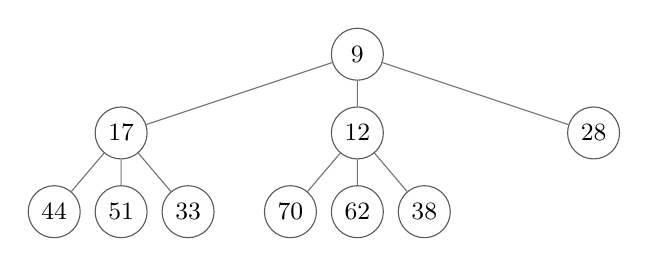
\begin{tikzpicture}[level distance=1.0cm,
    level 1/.style={sibling distance=3.0cm},
    level 2/.style={sibling distance=0.85cm},
    every node/.style={hpn}, edge from parent/.style={hpedge, draw}]
\node {9}
    child {node {17} child {node {44}} child {node {51}} child {node {33}}}
    child {node {12} child {node {70}} child {node {62}} child {node {38}}}
    child {node {28}};
\end{tikzpicture}
\diagcaption{建好的三元最小堆積。 每個節點最多三個子節點，$10$ 個元素的高度是 $3$，二
元堆積則是 $4$。}
\label{fig:hp-ternary}
\end{center}

實際的執行時間還和快取有關：$d$ 個子節點在陣列裡是相鄰的，一次讀進快取，樹又比較矮，所
以實務上常用 $d = 4$ 左右。

\section{雙端優先佇列、左傾樹與二項堆積}
\label{sec:hp-mergeable}

二元堆積有兩個做不到的地方。 第一，最小堆積找最大值要看所有的葉節點，$\Theta(n)$；想同時
取最小和最大，就要另外想辦法。 第二，兩個堆積合併成一個，只能把兩個陣列接起來重建，
$\Theta(n)$。 這一節的前三種結構（最小最大堆積、deap、對稱最小最大堆積）處理第一件，後兩
種（左傾樹、二項堆積）處理第二件。 每一種都以手算追蹤為主，考卷上最常見的題目就是「插入
（刪除）之後畫出結果」。

\subsection{最小最大堆積}

\textbf{雙端優先佇列}（double-ended priority queue）同時支援取出最小值和取出最大值。 例如
急診室同時想知道最緊急和最不緊急的病人，後者可以轉到一般門診。 \textbf{最小最大堆積}
（min-max heap）用一個陣列做到這件事。

\begin{definition}[最小最大堆積]
\label{def:hp-minmax}
最小最大堆積是存在陣列裡的完整二元樹，各層輪流是\textbf{最小層}和\textbf{最大層}：根所在
的深度 $0$ 是最小層，深度 $1$ 是最大層，深度 $2$ 又是最小層，依此類推。 最小層的節點
不大於它的所有子孫，最大層的節點不小於它的所有子孫。
\end{definition}

所以最小值在根，最大值是根的兩個子節點中較大的那個（只有一個元素時就是根）。 位置 $i$
的深度是 $\lfloor \lg i \rfloor$，偶數就在最小層。 和二元堆積不同的是，比較的對象常常
是\textbf{祖父}（位置 $\lfloor i/4 \rfloor$）和\textbf{孫子}，因為隔一層才是同一種層。

\textbf{插入}：新元素 $x$ 放在位置 $j = n + 1$，先和父節點比一次，決定它屬於「小的那一
邊」還是「大的那一邊」，之後只沿著同一種層的祖父往上走。

\begin{pseudo}[label=alg:hp-minmax-insert]{最小最大堆積的插入}
\Procedure{MinMax-Insert}{$A, x$}
    \State $A.\mathit{size} \gets A.\mathit{size} + 1$
    \State $j \gets A.\mathit{size}$
    \If{$j = 1$}
        \State $A[1] \gets x$
    \ElsIf{$j$ 在最小層}
        \If{$x > A[\lfloor j/2 \rfloor]$}
            \State $A[j] \gets A[\lfloor j/2 \rfloor]$ \Comment{父節點在最大層}
            \State \Call{Push-Up-Max}{$A, \lfloor j/2 \rfloor, x$}
        \Else
            \State \Call{Push-Up-Min}{$A, j, x$}
        \EndIf
    \Else \Comment{$j$ 在最大層}
        \If{$x < A[\lfloor j/2 \rfloor]$}
            \State $A[j] \gets A[\lfloor j/2 \rfloor]$ \Comment{父節點在最小層}
            \State \Call{Push-Up-Min}{$A, \lfloor j/2 \rfloor, x$}
        \Else
            \State \Call{Push-Up-Max}{$A, j, x$}
        \EndIf
    \EndIf
\EndProcedure
\Statex
\Procedure{Push-Up-Min}{$A, i, x$} \Comment{$i$ 在最小層，$x$ 要放在 $i$ 或它的祖先}
    \While{$i \ge 4$ \AND $x < A[\lfloor i/4 \rfloor]$}
        \State $A[i] \gets A[\lfloor i/4 \rfloor]$
        \State $i \gets \lfloor i/4 \rfloor$
    \EndWhile
    \State $A[i] \gets x$
\EndProcedure
\end{pseudo}

\proc{Push-Up-Max} 把第 19 行的 $<$ 改成 $>$。 這裡用「挖洞」的寫法：祖父往下挪，$x$ 最
後才放進去。 每一步往上兩層，所以插入只要 $O(\lg n)$，比較次數大約是 $\frac{1}{2}\lg n
+ 1$。

\textbf{取出最小值}：最小值在根。 把最後一個元素 $x$ 拿出來，堆積少一格，然後替 $x$ 在
根底下找位置。 根在最小層，要放的是「$x$ 和根的所有子孫中最小的」，而那個最小的一定在
根的子節點或孫節點裡（再往下的都被它們的祖先管住了）。

\begin{pseudo}[label=alg:hp-minmax-delete]{最小最大堆積的取出最小值}
\Function{MinMax-Extract-Min}{$A$} \Comment{假設 $A.\mathit{size} \ge 1$}
    \State $\mathit{min} \gets A[1]$
    \State $x \gets A[A.\mathit{size}]$
    \State $A.\mathit{size} \gets A.\mathit{size} - 1$
    \State $i \gets 1$
    \While{$2i \le A.\mathit{size}$}
        \State $k \gets$ $i$ 的子節點和孫節點之中，值最小的位置
        \If{$x \le A[k]$}
            \State \Break
        \EndIf
        \State $A[i] \gets A[k]$
        \If{$k$ 是 $i$ 的子節點}
            \State $i \gets k$
            \State \Break
        \EndIf
        \If{$x > A[\lfloor k/2 \rfloor]$} \Comment{$k$ 的父節點在最大層}
            \State 交換 $x$ 和 $A[\lfloor k/2 \rfloor]$
        \EndIf
        \State $i \gets k$
    \EndWhile
    \If{$A.\mathit{size} \ge 1$}
        \State $A[i] \gets x$
    \EndIf
    \State \Return $\mathit{min}$
\EndFunction
\end{pseudo}

每一輪往下兩層，看最多六個位置，所以是 $O(\lg n)$。 第 11 行處理 $k$ 是子節點的情況。
$k$ 在最大層，它的子孫都不大於 $A[k]$；而 $A[k]$ 又是所有候選（包括 $k$ 的子節點）裡最小
的，所以 $k$ 如果有子孫，值都等於 $A[k]$。 這時 $x > A[k]$ 不小於 $k$ 的任何子孫，放在最
大層的 $k$ 是合法的，搬到 $i$ 的 $A[k]$ 也不大於 $i$ 的任何子孫，可以結束。 第 15 行的交
換是因為 $x$ 要往孫子那裡走，路上會經過最大層的 $A[\lfloor k/2 \rfloor]$，$x$ 比它大的
話就不能待在它底下，兩者對調。 取出最大值的做法對稱：最大值在位置 $2$ 或 $3$，從那裡開始，把「最小」都換成「最大」。

\textbf{手算追蹤}。 下圖 (a) 是一個有 $10$ 個元素的最小最大堆積，陣列是
\[
\langle 11, 46, 72, 31, 23, 58, 38, 36, 37, 34 \rangle.
\]
依序做三個操作：插入 $8$、插入 $77$、取出最小值。

\begin{center}
\begin{tikzpicture}
\foreach \y/\t in {0/min, -0.95/max, -1.9/min, -2.85/max}
    \node[hpidx, anchor=east] at (-3.3,\y) {\t};
\hpheap{0,0}{6.0}{11/n,46/n,72/n,31/n,23/n,58/n,38/n,36/n,37/n,34/n}{m}
\hpheap{7.2,0}{6.0}{8/a,46/n,72/n,31/n,11/a,58/n,38/n,36/n,37/n,34/n,23/a}{n}
\node[font=\small] at (0,-3.65) {(a) 開始};
\node[font=\small] at (7.2,-3.65) {(b) 插入 $8$};
\end{tikzpicture}

\begin{tikzpicture}
\foreach \y/\t in {0/min, -0.95/max, -1.9/min, -2.85/max}
    \node[hpidx, anchor=east] at (-3.3,\y) {\t};
\hpheap{0,0}{6.0}{8/n,46/n,77/a,31/n,11/n,58/n,38/n,36/n,37/n,34/n,23/n,72/a}{o}
\hpheap{7.2,0}{6.0}{11/a,72/a,77/n,31/n,23/a,58/n,38/n,36/n,37/n,34/n,46/a}{p}
\node[font=\small] at (0,-3.65) {(c) 插入 $77$};
\node[font=\small] at (7.2,-3.65) {(d) 取出最小值 $8$};
\end{tikzpicture}
\diagcaption{最小最大堆積的三個操作。 左邊標出每一層是最小層還是最大層，橘色是這一步改
變的位置。}
\label{fig:hp-minmax}
\end{center}

\begin{itemize}
\item \textbf{插入 $8$}：放在位置 $11$，深度 $3$，是最大層。 父節點 $A[5] = 23$ 在最小
層，$8 < 23$，所以 $23$ 挪到位置 $11$，$8$ 改走最小層：從位置 $5$ 看祖父 $A[1] = 11$，
$8 < 11$，$11$ 挪到位置 $5$，$8$ 到了根。
\item \textbf{插入 $77$}：放在位置 $12$，最大層。 父節點 $A[6] = 58$，$77 > 58$，不用和
父節點換，直接走最大層：祖父 $A[3] = 72$，$77 > 72$，$72$ 挪到位置 $12$，$77$ 放在位
置 $3$。
\item \textbf{取出最小值}：取出 $8$，最後一個元素 $x = 72$ 拿出來。 根的子孫中，子節點
$46, 77$ 和孫節點 $31, 11, 58, 38$ 裡最小的是 $A[5] = 11$（孫節點），搬到根。 $11$ 的父
節點 $A[2] = 46$ 在最大層，$x = 72 > 46$，對調，$46$ 繼續往下找位置，$72$ 留在
$A[2]$。 到了位置 $5$，它的子節點 $34, 23$ 裡最小的是 $A[11] = 23$（子節點），比 $46$
小，$23$ 搬到位置 $5$，$46$ 放進位置 $11$，結束。
\end{itemize}

最後的陣列是 $\langle 11, 72, 77, 31, 23, 58, 38, 36, 37, 34, 46 \rangle$。 可以逐層檢查：
最大層的 $72$ 不小於它底下的 $31, 23, 36, 37, 34, 46$，最小層的 $23$ 不大於 $34, 46$。

\subsection{雙端堆積（deap）}
\label{sec:hp-deap}

最小最大堆積把小的和大的放在交錯的層裡。 \textbf{deap}（double-ended heap，中文常叫雙端
堆積）改成左右分開：根不放元素，根的左子樹是一個最小堆積，右子樹是一個最大堆積，兩邊再用
「對應點」互相約束，保證左邊每個元素都不大於右邊對應位置的元素。

仍然用陣列存。 $A[1]$ 是空的根，元素放在 $A[2..\mathit{last}]$，共 $\mathit{last} - 1$ 個。 深度
$d \ge 1$ 的位置是 $2^d$ 到 $2^{d+1} - 1$，前一半屬於最小堆積，後一半屬於最大堆積：位置 $i$
在最大堆積，若且唯若 $i \ge 2^d + 2^{d-1}$，其中 $d = \lfloor \lg i \rfloor$。 兩個堆積的根分別是
$A[2]$ 和 $A[3]$；除了這兩個根，每個位置的父節點仍然是 $\lfloor i/2 \rfloor$，而且和自己在同
一邊。

\begin{definition}[deap]
\label{def:hp-deap}
deap 是存在陣列 $A[1..\mathit{last}]$ 的完整二元樹，根 $A[1]$ 不放元素，而且滿足：
\begin{enumerate}
\item 根的左子樹是最小堆積，右子樹是最大堆積（只有一個元素時右子樹是空的）。
\item 對最小堆積的每個位置 $i$，令 $j = i + 2^{\lfloor \lg i \rfloor - 1}$，這是最大堆積裡同一層、
同一個相對位置的\textbf{對應點}；如果 $j > \mathit{last}$，改用它的父節點 $\lfloor j/2 \rfloor$。
那麼 $A[i] \le A[j]$。
\end{enumerate}
\end{definition}

改用父節點是因為最後一層從左邊填起，最小堆積那一邊的最後一層可能比右邊多出幾個節點，它們
在右邊還沒有對應點，就和那個位置的父節點比。 反過來，最大堆積的位置 $j$ 的對應點是
$i = j - 2^{\lfloor \lg j \rfloor - 1}$，這個 $i$ 一定存在。

最小值在 $A[2]$，最大值在 $A[3]$（只有一個元素時兩者都是 $A[2]$）。 $A[2]$ 是最小堆積的最
小值；最大堆積的任何位置 $j$，對應點 $i$ 都存在而且 $A[i] \le A[j]$，所以 $A[j]$ 也不小於
$A[2]$。 $A[3]$ 是最大值的理由對稱。

\textbf{插入}。 新元素 $x$ 先放在新的最後一格 $p$。 如果 $p$ 在最小堆積，看它的對應點 $j$：
$x > A[j]$ 表示 $x$ 屬於大的那一邊，把 $A[j]$ 搬到 $p$，$x$ 從 $j$ 開始在最大堆積裡上浮；否則
$x$ 從 $p$ 開始在最小堆積裡上浮。 $p$ 在最大堆積時反過來，和對應點比，$x$ 比較小就換到最小
堆積那一邊。 上浮用最小最大堆積那種「挖洞」的寫法：\proc{Min-Up}$(A, i, x)$ 從位置 $i$ 沿著父
節點往上，父節點比 $x$ 大就把父節點往下挪，最多走到最小堆積的根 $A[2]$；\proc{Max-Up} 對稱，
最多走到 $A[3]$。 新的最後一格 $p$ 在最小堆積時，它的對應點一定超出範圍，改用的
$\lfloor j/2 \rfloor$ 正好是 $p$ 的父節點的對應點，所以搬到 $p$ 的 $A[j]$ 不小於 $p$ 的父節點，
最小堆積的性質不會被破壞。

\textbf{取出最小值}。 最小值在 $A[2]$。 把最後一格的元素 $x$ 拿出來，$\mathit{last}$ 減 $1$。
接著讓 $A[2]$ 這個洞沿著最小堆積往下走：每次把較小的子節點搬上來，直到洞到了沒有子節點的
位置 $i$。 最後把 $x$ 放進位置 $i$，做法和插入時一樣，先和 $i$ 的對應點比。 和二元堆積的
下沉不同，洞不在中途停下來，一路走到最底：這樣 $x$ 只需要在最後決定去哪一邊，再往上浮一次。

\textbf{取出最大值}。 對稱：最大值在 $A[3]$（只有一個元素時就是 $A[2]$），洞沿著最大堆積較
大的子節點走到底，到了位置 $j$ 再放 $x$。 這時有一個細節：如果對應點 $i$ 有子節點，這些子節
點在最大堆積那邊沒有對應點，依定義都要和 $j$ 比，所以 $x$ 要和「$i$ 的子節點中較大的那個」比，
不能只和 $A[i]$ 比。

\begin{pseudo}[label=alg:hp-deap]{deap 的插入與取出最小值}
\Procedure{Deap-Insert}{$A, x$}
    \State $A.\mathit{last} \gets A.\mathit{last} + 1$
    \If{$A.\mathit{last}$ 在最大堆積}
        \State \Call{Deap-Put-Max}{$A, A.\mathit{last}, x$}
    \Else
        \State \Call{Deap-Put-Min}{$A, A.\mathit{last}, x$}
    \EndIf
\EndProcedure
\Statex
\Procedure{Deap-Put-Min}{$A, i, x$} \Comment{位置 $i$ 在最小堆積，目前是空的}
    \State $j \gets i + 2^{\lfloor \lg i \rfloor - 1}$ \Comment{對應點}
    \If{$j > A.\mathit{last}$}
        \State $j \gets \lfloor j/2 \rfloor$ \Comment{最大堆積是空的時 $j = 1$}
    \EndIf
    \If{$j \ge 3$ \AND $x > A[j]$}
        \State $A[i] \gets A[j]$
        \State \Call{Max-Up}{$A, j, x$}
    \Else
        \State \Call{Min-Up}{$A, i, x$}
    \EndIf
\EndProcedure
\Statex
\Procedure{Deap-Put-Max}{$A, j, x$} \Comment{位置 $j$ 在最大堆積，目前是空的}
    \State $i \gets j - 2^{\lfloor \lg j \rfloor - 1}$ \Comment{對應點}
    \If{$2i \le A.\mathit{last}$} \Comment{$i$ 有子節點：改看較大的子節點}
        \State $i \gets 2i$
        \If{$i + 1 \le A.\mathit{last}$ \AND $A[i + 1] > A[i]$}
            \State $i \gets i + 1$
        \EndIf
    \EndIf
    \If{$x < A[i]$}
        \State $A[j] \gets A[i]$
        \State \Call{Min-Up}{$A, i, x$}
    \Else
        \State \Call{Max-Up}{$A, j, x$}
    \EndIf
\EndProcedure
\Statex
\Function{Deap-Delete-Min}{$A$} \Comment{假設 $A.\mathit{last} \ge 2$}
    \State $\mathit{min} \gets A[2]$
    \State $x \gets A[A.\mathit{last}]$
    \State $A.\mathit{last} \gets A.\mathit{last} - 1$
    \If{$A.\mathit{last} \ge 2$}
        \State $i \gets 2$
        \While{$2i \le A.\mathit{last}$} \Comment{洞沿著較小的子節點走到底}
            \State $c \gets 2i$
            \If{$c + 1 \le A.\mathit{last}$ \AND $A[c + 1] < A[c]$}
                \State $c \gets c + 1$
            \EndIf
            \State $A[i] \gets A[c]$
            \State $i \gets c$
        \EndWhile
        \State \Call{Deap-Put-Min}{$A, i, x$}
    \EndIf
    \State \Return $\mathit{min}$
\EndFunction
\end{pseudo}

\proc{Deap-Delete-Max} 把 \proc{Deap-Delete-Min} 的 $A[2]$ 換成 $A[3]$（只有一個元素時直接
取 $A[2]$）、「較小的子節點」換成「較大的子節點」，最後呼叫 \proc{Deap-Put-Max}。 樹高是
$\lfloor \lg \mathit{last} \rfloor + 1$，洞往下走和上浮都只沿一條路徑，所以三個操作都是
$O(\lg n)$。

\textbf{手算追蹤}。 把 $35, 69, 29, 33, 65, 52, 96, 61, 24, 14, 55$ 依序插入空的 deap，再取出最
小值、取出最大值。 下表每一列是操作之後的 $A[2..12]$，粗體的位置屬於最大堆積。

\begin{center}
\small
\begin{tabular}{l*{11}{c}}
\toprule
操作 & 2 & \textbf{3} & 4 & 5 & \textbf{6} & \textbf{7} & 8 & 9 & 10 & 11 & \textbf{12} \\
\midrule
插入 35 & 35 \\
插入 69 & 35 & 69 \\
插入 29 & 29 & 69 & 35 \\
插入 33 & 29 & 69 & 35 & 33 \\
插入 65 & 29 & 69 & 35 & 33 & 65 \\
插入 52 & 29 & 69 & 35 & 33 & 65 & 52 \\
插入 96 & 29 & 96 & 35 & 33 & 69 & 52 & 65 \\
插入 61 & 29 & 96 & 35 & 33 & 69 & 52 & 65 & 61 \\
插入 24 & 24 & 96 & 35 & 29 & 69 & 52 & 65 & 61 & 33 \\
插入 14 & 14 & 96 & 35 & 24 & 69 & 52 & 65 & 61 & 33 & 29 \\
插入 55 & 14 & 96 & 35 & 24 & 69 & 52 & 55 & 61 & 33 & 29 & 65 \\
\midrule
取出最小 14 & 24 & 96 & 35 & 29 & 69 & 65 & 55 & 61 & 33 & 52 \\
取出最大 96 & 24 & 69 & 35 & 29 & 61 & 65 & 55 & 52 & 33 \\
\bottomrule
\end{tabular}
\end{center}

\begin{itemize}
\item \textbf{插入 $29$}：放在位置 $4$（最小堆積）。 對應點 $4 + 2 = 6$ 超出範圍，改用父節點
$3$；$29 \le A[3] = 69$，留在最小堆積上浮，$A[2] = 35$ 比它大，$35$ 往下挪，$29$ 到位置 $2$。
\item \textbf{插入 $96$}：放在位置 $8$（深度 $3$ 的 $8$ 到 $11$ 屬於最小堆積）。 對應點 $12$ 超出
範圍，改用 $6$；$96 > A[6] = 65$，所以 $65$ 搬到位置 $8$，$96$ 從位置 $6$ 在最大堆積上浮，父節
點 $A[3] = 69$ 比它小，$69$ 往下挪，$96$ 到位置 $3$。
\item \textbf{插入 $55$}：放在位置 $12$（最大堆積）。 對應點 $12 - 4 = 8$，它沒有子節點；
$55 < A[8] = 65$，所以 $65$ 搬到位置 $12$，$55$ 從位置 $8$ 在最小堆積上浮，父節點 $A[4] = 35$
比它小，停。
\item \textbf{取出最小值 $14$}：最後一格的 $65$ 拿出來。 洞從位置 $2$ 往下：子節點 $35, 24$ 中
較小的 $24$ 上來，洞到位置 $5$；子節點 $33, 29$ 中較小的 $29$ 上來，洞到位置 $11$，沒有子
節點了。 位置 $11$ 的對應點 $15$ 超出範圍，改用 $7$；$65 > A[7] = 52$，所以 $52$ 搬到位置
$11$，$65$ 從位置 $7$ 上浮，父節點 $96$ 比它大，停在 $7$。
\item \textbf{取出最大值 $96$}：最後一格的 $52$ 拿出來。 洞從位置 $3$ 往下：子節點 $69, 65$ 中
較大的 $69$ 上來，洞到位置 $6$，沒有子節點了。 對應點 $6 - 2 = 4$ 有子節點 $55, 61$，取較大的
$61$（位置 $9$）；$52 < 61$，所以 $61$ 搬到位置 $6$，$52$ 從位置 $9$ 在最小堆積上浮，父節點
$35$ 比它小，停。
\end{itemize}

最後一步如果只和 $A[4] = 35$ 比，$52$ 會留在位置 $6$；位置 $9$ 的 $61$ 對應點 $13$ 超出範圍，改
用 $6$，就違反了 $61 \le 52$。 這就是 \proc{Deap-Put-Max} 要看子節點的原因。

\begin{center}
\begin{tikzpicture}
\hpshowidxtrue
\hpheap{0,0}{6.0}{/e,14/n,96/n,35/n,24/n,69/n,52/n,55/n,61/n,33/n,29/n,65/n}{da}
\hpshowidxfalse
\node[hpidx] at (-1.5,-3.35) {最小堆積};
\node[hpidx] at (1.5,-3.35) {最大堆積};
\hpheap{7.2,0}{6.0}{/e,24/a,96/n,35/n,29/a,69/n,65/a,55/n,61/n,33/n,52/a}{db}
\node[font=\small] at (0,-3.9) {(a) 插入 $11$ 個之後};
\node[font=\small] at (7.2,-3.9) {(b) 取出最小值 $14$};
\end{tikzpicture}

\begin{tikzpicture}
\hpheap{0,0}{6.0}{/e,24/n,69/a,35/n,29/n,61/a,65/n,55/n,52/a,33/n}{dc}
\node[font=\small] at (0,-3.9) {(c) 取出最大值 $96$};
\end{tikzpicture}
\diagcaption{deap 的三個狀態。 虛線圓是不放元素的根，左子樹是最小堆積，右子樹是最大堆積；
(a) 右上角的小字是陣列位置，橘色是上一個狀態之後改變的位置。}
\label{fig:hp-deap}
\end{center}

\begin{examnote}
deap 的題目先確認三件事。 一、根是空的，元素從 $A[2]$ 開始；有的書把 $A[2]$ 叫做「位置 1」，
對應點的公式要跟著平移，照題目給的圖和編號。 二、對應點超出範圍時改用父節點。 三、取出最
大值時，要和「對應點的較大子節點」比（對應點沒有子節點才和對應點本身比）。 例如依序插入
$10, 30, 40, 20$ 得到 $A[2..5] = \langle 10, 40, 30, 20 \rangle$，取出最大值 $40$ 時，$20$ 要和
$A[4] = 30$ 比，結果是 $\langle 10, 30, 20 \rangle$；只和 $A[2] = 10$ 比會得到
$\langle 10, 20, 30 \rangle$，位置 $4$ 的 $30$ 比它的對應點 $A[3] = 20$ 大，不是 deap。
層數照全書約定從根算第 $1$ 層，所以 $A[2]$、$A[3]$ 在第 $2$ 層。
\end{examnote}

\subsection{對稱最小最大堆積}
\label{sec:hp-smmh}

\textbf{對稱最小最大堆積}（symmetric min-max heap，簡稱 SMMH）也是根不放元素的完整二元樹，
但規則只看兄弟和祖父，不用算對應點，所以程式比 deap 短。

\begin{definition}[對稱最小最大堆積]
\label{def:hp-smmh}
存在陣列 $A[1..\mathit{last}]$ 的完整二元樹，根 $A[1]$ 不放元素，其他每個節點放一個元素，而且：
\begin{enumerate}
\item[P1.] 每個有右兄弟的節點，元素不大於右兄弟：偶數位置 $x$ 有 $A[x] \le A[x + 1]$。
\item[P2.] 每個有祖父 $g$ 的節點 $x$，$A[2g] \le A[x]$：祖父的左子節點不大於它。
\item[P3.] 每個有祖父 $g$ 的節點 $x$，$A[2g + 1] \ge A[x]$：祖父的右子節點不小於它。
\end{enumerate}
\end{definition}

換個方式讀：任何一個節點 $y$，把 $y$ 的子樹扣掉 $y$ 自己，剩下的元素裡最小的在 $y$ 的左子節
點，最大的在 $y$ 的右子節點。 （P1 管左右子節點本身，P2、P3 管下面兩層，再往下一層一層套
用就得到整棵子樹。） 拿根當 $y$，最小值在 $A[2]$，最大值在 $A[3]$。

\textbf{插入}。 新元素 $x$ 放在新的最後一格 $c$。 如果 $c$ 是右子節點而 $x$ 比左兄弟小，會違反
P1，所以先把左兄弟搬到 $c$，$x$ 改看左兄弟的位置。 接著只要 $c$ 有祖父 $g$（$c \ge 4$），就和
$A[2g]$、$A[2g + 1]$ 比：比 $A[2g]$ 小就把它搬下來、$x$ 往上到 $2g$；比 $A[2g + 1]$ 大就把它
搬下來、$x$ 往上到 $2g + 1$；介於兩者之間就停。 每一步往上一層。

\textbf{取出最小值}。 最小值在 $A[2]$。 把最後一格的元素 $y$ 拿出來，替 $y$ 從洞 $e = 2$ 往下
找位置。 洞 $e$ 一定是左子節點；扣掉它以後，$e$ 和右兄弟 $e + 1$ 底下（不含 $e + 1$ 本身）最
小的元素，依上面的讀法一定是 $A[2e]$ 或 $A[2e + 2]$，也就是 $e$ 和 $e + 1$ 的左子節點。 取兩者
中較小的 $k$：$y \le A[k]$ 就把 $y$ 放在 $e$；否則 $A[k]$ 上來，洞移到 $k$。 洞移到新位置之後，
$y$ 將來會放在這個洞或它底下，要先檢查 P1：$y$ 比新洞的右兄弟大，就和右兄弟的元素對調，
帶著比較小的那個繼續往下。

\begin{pseudo}[label=alg:hp-smmh]{對稱最小最大堆積的插入與取出最小值}
\Procedure{SMMH-Insert}{$A, x$}
    \State $A.\mathit{last} \gets A.\mathit{last} + 1$
    \State $c \gets A.\mathit{last}$
    \If{$c$ 是奇數 \AND $x < A[c - 1]$} \Comment{P1：比左兄弟小}
        \State $A[c] \gets A[c - 1]$
        \State $c \gets c - 1$
    \EndIf
    \While{$c \ge 4$}
        \State $g \gets \lfloor c/4 \rfloor$ \Comment{祖父}
        \If{$x < A[2g]$} \Comment{P2}
            \State $A[c] \gets A[2g]$
            \State $c \gets 2g$
        \ElsIf{$x > A[2g + 1]$} \Comment{P3}
            \State $A[c] \gets A[2g + 1]$
            \State $c \gets 2g + 1$
        \Else
            \State \Break
        \EndIf
    \EndWhile
    \State $A[c] \gets x$
\EndProcedure
\Statex
\Function{SMMH-Delete-Min}{$A$} \Comment{假設 $A.\mathit{last} \ge 2$}
    \State $\mathit{min} \gets A[2]$
    \State $y \gets A[A.\mathit{last}]$
    \State $A.\mathit{last} \gets A.\mathit{last} - 1$
    \If{$A.\mathit{last} \ge 2$}
        \State $e \gets 2$ \Comment{洞，一定是左子節點}
        \While{$2e \le A.\mathit{last}$}
            \State $k \gets 2e$
            \If{$2e + 2 \le A.\mathit{last}$ \AND $A[2e + 2] < A[2e]$}
                \State $k \gets 2e + 2$
            \EndIf
            \If{$y \le A[k]$}
                \State \Break
            \EndIf
            \State $A[e] \gets A[k]$
            \State $e \gets k$
            \If{$e + 1 \le A.\mathit{last}$ \AND $y > A[e + 1]$} \Comment{P1}
                \State 交換 $y$ 和 $A[e + 1]$
            \EndIf
        \EndWhile
        \State $A[e] \gets y$
    \EndIf
    \State \Return $\mathit{min}$
\EndFunction
\end{pseudo}

\proc{SMMH-Delete-Max} 對稱：最大值在 $A[3]$（只有一個元素時是 $A[2]$），洞 $e$ 一定是右子
節點，候選是 $e - 1$ 和 $e$ 的子節點中最大的（右子節點存在就是右子節點，否則是左子節點），
洞移下去之後檢查 $y$ 有沒有比新洞的左兄弟小。 插入每層比兩次，取出每層最多比三次（兩個候
選、$y$、兄弟），都是 $O(\lg n)$。

\textbf{手算追蹤}。 用和 deap 相同的輸入 $35, 69, 29, 33, 65, 52, 96, 61, 24, 14, 55$，再取出最
小值和最大值。

\begin{center}
\small
\begin{tabular}{l*{11}{c}}
\toprule
操作 & 2 & 3 & 4 & 5 & 6 & 7 & 8 & 9 & 10 & 11 & 12 \\
\midrule
插入 35 & 35 \\
插入 69 & 35 & 69 \\
插入 29 & 29 & 69 & 35 \\
插入 33 & 29 & 69 & 33 & 35 \\
插入 65 & 29 & 69 & 33 & 35 & 65 \\
插入 52 & 29 & 69 & 33 & 35 & 52 & 65 \\
插入 96 & 29 & 96 & 33 & 69 & 52 & 65 & 35 \\
插入 61 & 29 & 96 & 33 & 69 & 52 & 65 & 35 & 61 \\
插入 24 & 24 & 96 & 29 & 69 & 52 & 65 & 35 & 61 & 33 \\
插入 14 & 14 & 96 & 24 & 69 & 52 & 65 & 35 & 61 & 29 & 33 \\
插入 55 & 14 & 96 & 24 & 69 & 52 & 65 & 35 & 61 & 29 & 33 & 55 \\
\midrule
取出最小 14 & 24 & 96 & 29 & 69 & 52 & 65 & 35 & 61 & 33 & 55 \\
取出最大 96 & 24 & 69 & 29 & 61 & 52 & 65 & 35 & 55 & 33 \\
\bottomrule
\end{tabular}
\end{center}

\begin{itemize}
\item \textbf{插入 $33$}：位置 $5$ 是右子節點，比左兄弟 $35$ 小，$35$ 搬到位置 $5$，$33$ 改看位
置 $4$。 祖父是根，它的兩個子節點是 $29$ 和 $69$，$29 \le 33 \le 69$，停在位置 $4$。
\item \textbf{插入 $96$}：位置 $8$ 的祖父是 $2$，看 $A[4] = 33$、$A[5] = 35$；$96 > 35$，$35$ 搬
下來，$96$ 到位置 $5$。 位置 $5$ 的祖父是根，看 $A[2] = 29$、$A[3] = 69$；$96 > 69$，$69$ 搬下
來，$96$ 到位置 $3$。
\item \textbf{插入 $14$}：位置 $11$ 是右子節點，比左兄弟 $33$ 小，先換到位置 $10$。 再往上兩
步：比 $A[4] = 29$ 小，$29$ 搬到位置 $10$；比 $A[2] = 24$ 小，$24$ 搬到位置 $4$，$14$ 到根的
左子節點。
\item \textbf{取出最小值 $14$}：最後一格的 $55$ 拿出來，洞在位置 $2$。 候選 $A[4] = 24$、
$A[6] = 52$，$24$ 較小而且比 $55$ 小，搬上來，洞到位置 $4$；右兄弟 $A[5] = 69$ 不比 $55$ 小，不
用對調。 候選 $A[8] = 35$、$A[10] = 29$，$29$ 上來，洞到位置 $10$；右兄弟 $A[11] = 33 < 55$，
對調，$55$ 放進位置 $11$，手上換成 $33$。 位置 $10$ 沒有子節點，$33$ 放進去。
\item \textbf{取出最大值 $96$}：最後一格的 $55$ 拿出來，洞在位置 $3$。 候選是位置 $2$ 的右子節
點 $A[5] = 69$ 和位置 $3$ 的右子節點 $A[7] = 35$，$69$ 上來，洞到位置 $5$；左兄弟 $A[4] = 29$
不比 $55$ 大，不用對調。 候選是 $A[9] = 61$ 和 $A[10] = 33$（位置 $5$ 只有左子節點），$61$
上來，洞到位置 $9$，沒有子節點，$55$ 放進去。
\end{itemize}

\begin{center}
\begin{tikzpicture}
\hpshowidxtrue
\hpheap{0,0}{6.0}{/e,14/n,96/n,24/n,69/n,52/n,65/n,35/n,61/n,29/n,33/n,55/n}{sa}
\hpshowidxfalse
\hpheap{7.2,0}{6.0}{/e,24/a,96/n,29/a,69/n,52/n,65/n,35/n,61/n,33/a,55/a}{sb}
\node[font=\small] at (0,-3.65) {(a) 插入 $11$ 個之後};
\node[font=\small] at (7.2,-3.65) {(b) 取出最小值 $14$};
\end{tikzpicture}

\begin{tikzpicture}
\hpheap{0,0}{6.0}{/e,24/n,69/a,29/n,61/a,52/n,65/n,35/n,55/a,33/n}{sc}
\node[font=\small] at (0,-3.65) {(c) 取出最大值 $96$};
\end{tikzpicture}
\diagcaption{對稱最小最大堆積的三個狀態，輸入和圖~\ref{fig:hp-deap} 相同。 每一對兄弟都是
左小右大，而且夾住它們底下的所有元素。}
\label{fig:hp-smmh}
\end{center}

同樣的輸入，deap 和 SMMH 得到的陣列不一樣，兩個都是對的；考卷問哪一種，就照哪一種的規則
做。

\begin{examnote}
SMMH 的根也是空的，「第 $k$ 層」照全書約定從根算第 $1$ 層，最小值、最大值在第 $2$ 層。 插入
時先處理兄弟（P1），再一層一層和「祖父的兩個子節點」比，不要和根的兩個子節點比：例如
$A[2..10] = \langle 5, 50, 10, 40, 20, 30, 15, 35, 45 \rangle$ 的 $45$ 雖然不大於 $A[3] = 50$，
卻大於它祖父的右子節點 $A[5] = 40$，違反 P3。 取出時洞每往下一層，都要檢查一次兄弟。
\end{examnote}

\subsection{幾種雙端優先佇列的比較}
\label{sec:hp-depq}

還有一種常見的結構叫\textbf{區間堆積}（interval heap）：每個節點放兩個元素 $a \le b$，看成區間
$[a, b]$（最後一個節點可以只放一個），每個節點的區間都包含子節點的區間；所以根的 $a$ 是最小
值，$b$ 是最大值。 把 SMMH 去掉根、每一對兄弟合成一個節點，剛好就是區間堆積：P1 說每一對
左小右大，P2、P3 說底下的元素都夾在這一對之間。 例如圖~\ref{fig:hp-smmh} (a) 兩兩配對成
$[14, 96]$；$[24, 69]$、$[52, 65]$；$[35, 61]$、$[29, 33]$、$[55]$（分號隔開各層），每個區間
都包含它子節點的區間。 它的插入和取出和 SMMH
幾乎一樣，只是樹高少一層，這裡不再展開。

\begin{center}
\small
\begin{tabular}{>{\raggedright\arraybackslash}p{0.16\linewidth}>{\raggedright\arraybackslash}p{0.16\linewidth}>{\raggedright\arraybackslash}p{0.28\linewidth}>{\raggedright\arraybackslash}p{0.29\linewidth}}
\toprule
結構 & 最小、最大 & 插入 & 取出最小值 \\
\midrule
最小最大堆積 & $A[1]$；$A[2]$ 或 $A[3]$ & 和父節點比一次決定哪一種層，再沿祖父往上 &
看子節點和孫節點（最多六個），每次下兩層 \\
deap & $A[2]$；$A[3]$ & 和對應點比一次決定哪一邊，再在那一邊上浮 &
洞沿最小堆積走到底，再和對應點比 \\
SMMH & $A[2]$；$A[3]$ & 先和兄弟比，再和祖父的兩個子節點比 &
洞每層看兩個候選，再和兄弟比 \\
區間堆積 & 根的兩端 & 和 SMMH 相同，一個節點放兩個元素 & 和 SMMH 相同 \\
\bottomrule
\end{tabular}
\end{center}

四種的插入、取出最小值、取出最大值都是 $O(\lg n)$，找最小值和最大值都是 $\Theta(1)$。 deap 和
SMMH 多用一格空的根；SMMH 的規則最少，是最好寫的一種。

\subsection{左傾樹}

左傾樹的目的是\textbf{合併}（meld）：兩個優先佇列併成一個，只花 $O(\lg n)$。 它不再是完
整二元樹，改用節點和指標存，形狀可以很不平衡，但\textbf{右邊}一定很短。

對每個節點 $x$，令 $s(x)$ 是從 $x$ 往下走到最近的空位（\NIL）要經過幾個節點：
$s(\NIL) = 0$，$s(x) = 1 + \min\bigl(s(x.\mathit{left}), s(x.\mathit{right})\bigr)$。 葉節點的
$s$ 是 $1$；只有一個子節點的節點，$s$ 也是 $1$。 實作時每個節點用一個欄位 $x.s$ 存
$s(x)$，$s(\NIL)$ 直接當成 $0$。

\begin{definition}[左傾樹]
\label{def:hp-leftist}
二元樹的每個節點 $x$ 都滿足 $s(x.\mathit{left}) \ge s(x.\mathit{right})$，叫\textbf{左傾樹}
（leftist tree）。 如果同時滿足最小堆積的性質（父節點不大於子節點），叫\textbf{最小左傾
樹}。
\end{definition}

左傾的條件讓 $s(x) = 1 + s(x.\mathit{right})$：一路往右走就是最短的那條路。

\begin{theorem}
\label{thm:hp-leftist}
左傾樹中，以 $x$ 為根的子樹至少有 $2^{s(x)} - 1$ 個節點，從 $x$ 一路往右走到 \NIL 剛好經
過 $s(x)$ 個節點。 因此 $n$ 個節點的左傾樹，最右邊的路徑最多有 $\lg(n + 1)$ 個節點。
\end{theorem}

\begin{proof}
由 $s$ 的定義，從 $x$ 往下走不到 $s(x)$ 步不會遇到 \NIL，所以 $x$ 底下的前 $s(x)$ 層（深
度 $0$ 到 $s(x) - 1$，相對於 $x$）都是滿的，至少 $1 + 2 + \cdots + 2^{s(x) - 1} = 2^{s(x)}
- 1$ 個節點。 第二句從 $s(x) = 1 + s(x.\mathit{right})$ 往下歸納即可。 把兩者合起來，
$n \ge 2^{s(\text{根})} - 1$，所以右邊的路徑長 $s(\text{根}) \le \lg(n + 1)$。
\end{proof}

\textbf{合併}兩棵最小左傾樹 $a$、$b$：根比較小的那棵當新的根，把它的右子樹和另一棵\textbf{遞
迴合併}，結果接回右邊；回來時如果右邊的 $s$ 比左邊大，左右對調，再更新 $s$。

\begin{pseudo}[label=alg:hp-meld]{合併兩棵最小左傾樹}
\Function{Meld}{$a, b$}
    \If{$a = \NIL$}
        \State \Return $b$
    \EndIf
    \If{$b = \NIL$}
        \State \Return $a$
    \EndIf
    \If{$b.\mathit{key} < a.\mathit{key}$}
        \State 交換 $a$ 和 $b$ \Comment{讓 $a$ 是根比較小的那棵}
    \EndIf
    \State $a.\mathit{right} \gets$ \Call{Meld}{$a.\mathit{right}, b$}
    \If{$s(a.\mathit{left}) < s(a.\mathit{right})$}
        \State 交換 $a.\mathit{left}$ 和 $a.\mathit{right}$
    \EndIf
    \State $a.s \gets s(a.\mathit{right}) + 1$
    \State \Return $a$
\EndFunction
\end{pseudo}

每一層遞迴都沿著 $a$ 或 $b$ 的右邊路徑往下走一步，所以遞迴的次數不超過兩條右邊路徑的長度
和，由定理~\ref{thm:hp-leftist} 是 $O(\lg n_a + \lg n_b) = O(\lg n)$。 有了合併，其他操作
都很簡單：\textbf{插入}是和只有一個節點的樹合併；\textbf{取出最小值}是拿掉根，把左右兩棵
子樹合併。 兩者都是 $O(\lg n)$。

\textbf{手算追蹤}。 下圖把 $A$、$B$ 兩棵最小左傾樹合併，節點右邊的小字是 $s$。 考卷上
的做法分兩步：先把兩條右邊路徑依鍵的大小合成一條，掛在右邊（圖 (c)）；再從下往上，遇
到左邊的 $s$ 比右邊小就對調左右，同時更新 $s$（圖 (d)）。 兩步的結果和虛擬碼的遞迴完
全一樣，只是把「往下」和「回來」分開畫。

\begin{center}
\tikzset{lt/.style={hpn, label={[hpidx, inner sep=1pt]east:#1}},
    ltlev/.style={level distance=0.95cm, edge from parent/.style={hpedge, draw},
        level 1/.style={sibling distance=2.0cm},
        level 2/.style={sibling distance=1.0cm},
        level 3/.style={sibling distance=0.75cm}}}
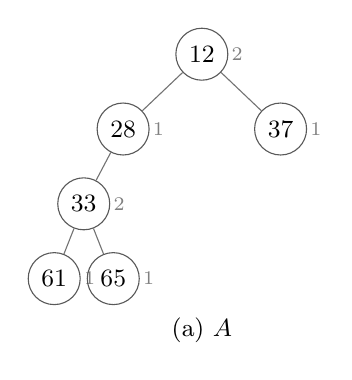
\begin{tikzpicture}[ltlev]
\node[lt=2] {12}
    child {node[lt=1] {28}
        child {node[lt=2] {33} child {node[lt=1] {61}} child {node[lt=1] {65}}}
        child[missing]}
    child {node[lt=1] {37}};
\node[font=\small] at (0,-3.5) {(a) $A$};
\end{tikzpicture}\hspace{1.2cm}%
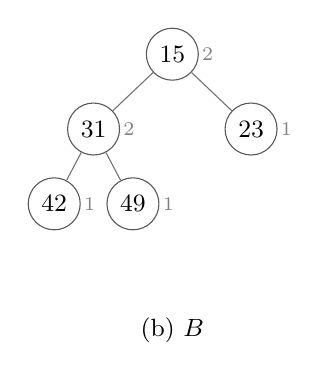
\begin{tikzpicture}[ltlev]
\node[lt=2] {15}
    child {node[lt=2] {31} child {node[lt=1] {42}} child {node[lt=1] {49}}}
    child {node[lt=1] {23}};
\node[font=\small] at (0,-3.5) {(b) $B$};
\end{tikzpicture}

\medskip
\begin{tikzpicture}[ltlev, level 1/.style={sibling distance=3.0cm},
    level 2/.style={sibling distance=1.5cm}]
\node[hpb] {12}
    child {node[lt=1] {28}
        child {node[lt=2] {33} child {node[lt=1] {61}} child {node[lt=1] {65}}}
        child[missing]}
    child {node[hpa] {15}
        child {node[lt=2] {31} child {node[lt=1] {42}} child {node[lt=1] {49}}}
        child {node[hpb] {23} child[missing] child {node[hpa] {37}}}};
\node[font=\small] at (0,-3.6) {(c) 右邊路徑合成一條};
\end{tikzpicture}\hspace{0.6cm}%
\begin{tikzpicture}[ltlev, level 1/.style={sibling distance=3.0cm},
    level 2/.style={sibling distance=1.5cm}]
\node[lt=2] {12}
    child {node[lt=2] {15}
        child {node[lt=2] {31} child {node[lt=1] {42}} child {node[lt=1] {49}}}
        child {node[lt=1] {23} child {node[lt=1] {37}} child[missing]}}
    child {node[lt=1] {28}
        child {node[lt=2] {33} child {node[lt=1] {61}} child {node[lt=1] {65}}}
        child[missing]};
\node[font=\small] at (0,-3.6) {(d) 對調之後};
\end{tikzpicture}
\diagcaption{合併兩棵最小左傾樹。 (c) 中有顏色的是合成之後的右邊路徑 $12, 15, 23, 37$：
粉紅色是左邊的 $s$ 比右邊小、回來時要對調的節點，橘色是不用對調的。}
\label{fig:hp-leftist}
\end{center}

合併的過程：$A$ 的右邊路徑是 $12, 37$，$B$ 的是 $15, 23$。 依大小合成
$12 \to 15 \to 23 \to 37$，每個節點保留自己原本的左子樹（圖 (c)）。 接著由下往上：
$37$ 是葉節點，$s = 1$；$23$ 的左邊是空的（$s = 0$）、右邊 $s = 1$，對調，$s(23) = 1$；
$15$ 的左邊 $s(31) = 2$ 不小於右邊 $s(23) = 1$，不用對調，$s(15) = 2$；$12$ 的左邊
$s(28) = 1$ 小於右邊 $s(15) = 2$，對調，$s(12) = 1 + s(28) = 2$。

接著取出最小值 $12$：把它的左右子樹（根是 $15$ 和 $28$）合併。 右邊路徑 $15, 23$ 和
$28$ 合成 $15 \to 23 \to 28$；由下往上，$23$ 左右的 $s$ 都是 $1$，不用對調，$s(23) =
2$；$15$ 左右都是 $2$，也不用對調。 結果是 $15$ 的左邊 $31(42, 49)$、右邊 $23$，$23$ 的
左邊 $37$、右邊 $28(33(61, 65), \NIL)$。

\begin{examnote}
$s$ 的定義各書不同。 有的書叫 shortest$(x)$，和本書一樣 $s(\NIL) = 0$；有的書叫 null path
length（npl），規定 $\mathrm{npl}(\NIL) = -1$、葉節點是 $0$，每個值都比本書小 $1$。 左傾的
條件和合併的做法不受影響，但算數值時要照題目的定義。 另外有一種\textbf{重量左傾樹}
（weight-biased leftist tree），比較的是子樹的節點個數而不是 $s$，見觀念題第~\ref{hp-q-wblt}~題。
\end{examnote}

\subsection{二項堆積}

二項堆積用另一種方式做到快速合併：把元素分成好幾棵形狀固定的樹，合併時像二進位加法一
樣處理同樣大小的樹。

\textbf{二項樹}（binomial tree）$B_k$ 遞迴定義：$B_0$ 是一個節點；$B_k$ 由兩棵 $B_{k-1}$
組成，其中一棵的根變成另一棵的根的最左邊的子節點。

\begin{center}
\tikzset{bt/.style={circle, draw=black!65, fill=black!12, minimum size=0.28cm, inner sep=0pt},
    btlev/.style={level distance=0.7cm, edge from parent/.style={hpedge, draw}}}
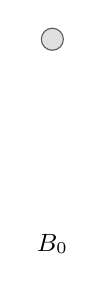
\begin{tikzpicture}[btlev]
\node[bt] {};
\node[font=\small] at (0,-2.6) {$B_0$};
\end{tikzpicture}\hspace{1.0cm}%
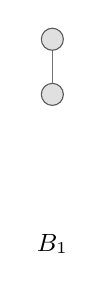
\begin{tikzpicture}[btlev]
\node[bt] {} child {node[bt] {}};
\node[font=\small] at (0,-2.6) {$B_1$};
\end{tikzpicture}\hspace{1.0cm}%
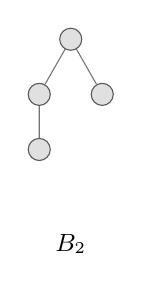
\begin{tikzpicture}[btlev, level 1/.style={sibling distance=0.8cm}]
\node[bt] {} child {node[bt] {} child {node[bt] {}}} child {node[bt] {}};
\node[font=\small] at (0,-2.6) {$B_2$};
\end{tikzpicture}\hspace{1.0cm}%
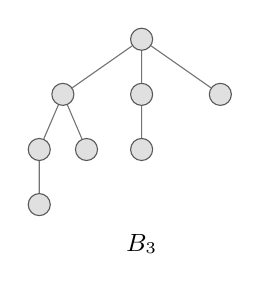
\begin{tikzpicture}[btlev, level 1/.style={sibling distance=1.0cm},
    level 2/.style={sibling distance=0.6cm}]
\node[bt] {}
    child {node[bt] {} child {node[bt] {} child {node[bt] {}}} child {node[bt] {}}}
    child {node[bt] {} child {node[bt] {}}}
    child {node[bt] {}};
\node[font=\small] at (0,-2.6) {$B_3$};
\end{tikzpicture}
\diagcaption{二項樹 $B_0$ 到 $B_3$。 $B_3$ 的根有三個子節點，由左到右是 $B_2$、$B_1$、
$B_0$ 的根。}
\label{fig:hp-binomial-trees}
\end{center}

從定義用歸納法可以得到 $B_k$ 的性質：

\begin{enumerate}
\item 有 $2^k$ 個節點，高度是 $k + 1$（最深的節點深度是 $k$）。
\item 深度 $d$ 的節點剛好有 $\binom{k}{d}$ 個。 （$B_k$ 深度 $d$ 的節點，來自一棵 $B_{k-1}$
的深度 $d$ 和另一棵 $B_{k-1}$ 的深度 $d - 1$，所以個數滿足巴斯卡公式
$\binom{k}{d} = \binom{k-1}{d} + \binom{k-1}{d-1}$，這也是「二項」的由來。）
\item 根的子節點數（叫\textbf{階數}，degree）是 $k$，比其他節點都多；根的子節點由左到右
是 $B_{k-1}, B_{k-2}, \ldots, B_0$ 的根。
\end{enumerate}

\textbf{二項堆積}（binomial heap）是一群二項樹，每棵都滿足最小堆積的性質，而且\textbf{同一個
階數最多一棵}。 $n$ 個元素的二項堆積有哪幾棵樹是固定的：把 $n$ 寫成二進位，第 $k$ 位是
$1$ 就有一棵 $B_k$。 例如 $n = 13 = 1101_2$，就是 $B_3$、$B_2$、$B_0$ 各一棵。 所以樹最多
$\lfloor \lg n \rfloor + 1$ 棵，每棵的階數不超過 $\lfloor \lg n \rfloor$，高度不超過
$\lfloor \lg n \rfloor + 1$。 各樹的
根用串列串起來，叫\textbf{根串列}（root list），依階數由小到大排。

每個節點的子節點個數不固定，所以用第~\ref{sec:bt-lcrs}~節的左孩子右兄弟存：
$x.\mathit{child}$ 指向最左邊的子節點，$x.\mathit{sibling}$ 指向右邊的下一個兄弟，另外
$x.p$ 指向父節點，$x.\mathit{degree}$ 記子節點個數。 根串列就是用各棵樹的根的
$\mathit{sibling}$ 串起來的。

基本的動作是把兩棵同階的樹連成一棵：根比較大的那棵掛到另一棵的根底下，成為最左邊的子
節點。 一棵 $B_k$ 和一棵 $B_k$ 連成 $B_{k+1}$，堆積性質仍然成立，$O(1)$。

\begin{pseudo}[label=alg:hp-binomial-link]{連結兩棵同階的二項樹}
\Function{Binomial-Link}{$y, z$} \Comment{$y$、$z$ 是同階的根}
    \If{$z.\mathit{key} < y.\mathit{key}$}
        \State 交換 $y$ 和 $z$
    \EndIf
    \State $z.p \gets y$
    \State $z.\mathit{sibling} \gets y.\mathit{child}$ \Comment{$z$ 變成 $y$ 最左邊的子節點}
    \State $y.\mathit{child} \gets z$
    \State $y.\mathit{degree} \gets y.\mathit{degree} + 1$
    \State \Return $y$
\EndFunction
\end{pseudo}

其他操作都從\textbf{合併}來：

\begin{itemize}
\item \textbf{合併}兩個二項堆積：從階數 $0$ 開始往上，像二進位加法。 每個階數 $k$ 可能有
$0$ 到 $3$ 棵樹（兩個堆積各一棵，加上前一位的進位）。 $0$ 或 $1$ 棵就留下；$2$ 棵就連成
一棵 $B_{k+1}$ 進位；$3$ 棵就留下一棵，另外兩棵連成進位。 根串列長 $O(\lg n)$，共
$O(\lg n)$。
\item \textbf{插入}：和只有一棵 $B_0$ 的堆積合併。 最壞要連結 $O(\lg n)$ 次（$n = 2^k - 1$
時一路進位），但這和第~3~章的二進位計數器一樣：連結的次數等於 $n$ 的二進位尾端連續的
$1$ 的個數，平攤只有 $O(1)$。 換個方式看，從空的堆積連續插入 $n$ 次，一共產生 $n$ 棵
$B_0$，每次連結讓樹少一棵，最後剩 $b(n)$ 棵，所以總共剛好連結 $n - b(n)$ 次。
\item \textbf{找最小值}：最小值一定是某棵樹的根，掃過根串列，$O(\lg n)$（另外記一個指向
最小根的指標，就是 $O(1)$）。
\item \textbf{取出最小值}：找到最小的根，從根串列拿掉；它的子節點由左到右是
$B_{k-1}, \ldots, B_0$，反過來排就是一個合法的二項堆積，再和剩下的堆積合併。
$O(\lg n)$。
\item \textbf{減少鍵值}：在那棵樹裡像二元堆積一樣往上換，樹高 $O(\lg n)$。 \textbf{刪除}
任意元素：把它的鍵減成 $-\infty$，再取出最小值。
\end{itemize}

\textbf{手算追蹤}。 把 $27, 13, 41, 8, 35, 19, 50$ 依序插入空的二項堆積，再取出最小值。
下表的「之後」用 $r[\,\cdots]$ 表示根是 $r$、方括號裡由左到右是它的子樹。

\begin{center}
\begin{tabular}{lccl}
\toprule
插入 & 插入前的 $n$ & 連結次數 & 之後的根串列 \\
\midrule
27 & $0 = 000_2$ & 0 & $B_0{:}\,27$ \\
13 & $1 = 001_2$ & 1 & $B_1{:}\,13[27]$ \\
41 & $2 = 010_2$ & 0 & $B_0{:}\,41$，$B_1{:}\,13[27]$ \\
8 & $3 = 011_2$ & 2 & $B_2{:}\,8[13[27],\,41]$ \\
35 & $4 = 100_2$ & 0 & $B_0{:}\,35$，$B_2{:}\,8[13[27],\,41]$ \\
19 & $5 = 101_2$ & 1 & $B_1{:}\,19[35]$，$B_2{:}\,8[13[27],\,41]$ \\
50 & $6 = 110_2$ & 0 & $B_0{:}\,50$，$B_1{:}\,19[35]$，$B_2{:}\,8[13[27],\,41]$ \\
\bottomrule
\end{tabular}
\end{center}

插入 $8$ 時，$B_0{:}\,8$ 和 $B_0{:}\,41$ 連成 $B_1{:}\,8[41]$，進位後和 $B_1{:}\,13[27]$ 連
成 $B_2$，根是較小的 $8$，$13$ 那棵掛在最左邊。 連結次數總共 $4 = 7 - b(7)$。

取出最小值 $8$：它的子樹 $B_1{:}\,13[27]$、$B_0{:}\,41$ 自成一個堆積，和剩下的
$\{B_0{:}\,50,\ B_1{:}\,19[35]\}$ 合併。 階數 $0$ 有 $50$、$41$ 兩棵，連成 $41[50]$ 進位；
階數 $1$ 有 $19[35]$、$13[27]$ 和進位的 $41[50]$ 三棵，留下進位的那棵，另外兩棵連成
$13[19[35],\,27]$ 進位到階數 $2$。 結果是 $6 = 110_2$ 個元素，兩棵樹。

\begin{center}
\tikzset{btlev/.style={level distance=0.9cm, edge from parent/.style={hpedge, draw},
    level 1/.style={sibling distance=1.0cm}}}
\begin{tikzpicture}[btlev]
\node[hpn] (r0) at (0,0) {50};
\node[hpn] (r1) at (1.3,0) {19} child {node[hpn] {35}};
\node[hpn] (r2) at (3.3,0) {8} child {node[hpn] {13} child {node[hpn] {27}}}
    child {node[hpn] {41}};
\draw[densely dashed, black!50] (r0) -- (r1) -- (r2);
\node[font=\small] at (1.8,-2.6) {(a) 插入 $7$ 個之後};
\end{tikzpicture}\hspace{1.4cm}%
\begin{tikzpicture}[btlev]
\node[hpn] (s1) at (0,0) {41} child {node[hpn] {50}};
\node[hpn] (s2) at (2.0,0) {13} child {node[hpn] {19} child {node[hpn] {35}}}
    child {node[hpn] {27}};
\draw[densely dashed, black!50] (s1) -- (s2);
\node[font=\small] at (1.2,-2.6) {(b) 取出 $8$ 之後};
\end{tikzpicture}
\diagcaption{二項堆積。 虛線是根串列，依階數由小到大。}
\label{fig:hp-binomial-heap}
\end{center}

\begin{examnote}
合併時某個階數有三棵樹，留哪一棵、連哪兩棵，各書的規定不同，結果都是合法的二項堆積，
但形狀不一樣。 作答時寫明你的規則（本書留下進位來的那棵）。 另外有的書把二項堆積寫成
「延遲合併」的版本：插入和合併只把根串列接起來，$O(1)$，等到取出最小值時才把同階的樹
兩兩連結。 如果題目的圖裡有兩棵同階的樹，就是這個版本，取出最小值時要把所有同階的樹
連到每個階數只剩一棵為止。 下一節的費氏堆積就是從延遲合併的版本再往前走一步。
\end{examnote}

\section{費氏堆積的平攤成本}
\label{sec:hp-fib}

前面的堆積，\proc{Decrease-Key} 都是 $O(\lg n)$。 Dijkstra 演算法在邊很多的圖上會做
$\Theta(m)$ 次 \proc{Decrease-Key}，卻只做 $n$ 次 \proc{Extract-Min}；如果
\proc{Decrease-Key} 能變成 $O(1)$，總時間就能從 $O(m \lg n)$ 降到 $O(m + n \lg n)$。
\textbf{費氏堆積}（Fibonacci heap）做到了這件事，不過是\textbf{平攤}的 $O(1)$。 這一節只
講它怎麼做、各操作的平攤成本是多少，以及怎麼用第~3~章的位能法得到這些結果，不做逐步
追蹤。

\subsection{結構與操作}

費氏堆積也是一群滿足最小堆積性質的樹，根用環狀雙向串列串起來，另外有一個指標指向最小
的根。 和二項堆積相比，它更懶：

\begin{itemize}
\item \textbf{插入}：新節點直接加進根串列，必要時更新最小指標。 不做任何連結。
\item \textbf{合併}：兩個根串列接起來，最小指標取兩者較小的。
\item \textbf{取出最小值}：拿掉最小的根，它的子節點都加進根串列；然後\textbf{整理}
（consolidate）根串列，把同階數的樹兩兩連結，直到每個階數只剩一棵，順便找出新的最
小值。 插入、合併時沒做的連結，都留到這一步才做。
\item \textbf{減少鍵值}：鍵變小以後如果比父節點小，就把這個節點連同它的子樹\textbf{剪
下來}，放進根串列。 為了不讓樹被剪得太稀疏，每個節點有一個標記：非根的節點第一次失去
子節點時做標記；已經有標記的節點再失去一個子節點，自己也被剪下來，再往上檢查它的父節
點，這叫\textbf{連鎖剪下}（cascading cut）。
\item \textbf{刪除}：減少鍵值到 $-\infty$，再取出最小值。
\end{itemize}

連鎖剪下保證一個階數是 $k$ 的節點，子樹至少有 $F_{k+2} \ge \phi^k$ 個節點，$F$ 是費氏數、
$\phi = (1 + \sqrt{5})/2$（名字就是這麼來的）。 所以 $n$ 個節點的費氏堆積，最大的階數
$D(n) \le \log_\phi n = O(\lg n)$。 這個結論這裡不證明，只拿來用。

\subsection{平攤成本}

\begin{center}
\begin{tabular}{lccc}
\toprule
操作 & 二元堆積（最壞） & 二項堆積（最壞） & 費氏堆積（平攤） \\
\midrule
\proc{Insert} & $O(\lg n)$ & $O(\lg n)$ & $O(1)$ \\
\proc{Minimum} & $\Theta(1)$ & $O(\lg n)$ & $O(1)$ \\
\proc{Extract-Min} & $O(\lg n)$ & $O(\lg n)$ & $O(\lg n)$ \\
合併 & $\Theta(n)$ & $O(\lg n)$ & $O(1)$ \\
\proc{Decrease-Key} & $O(\lg n)$ & $O(\lg n)$ & $O(1)$ \\
\proc{Delete} & $O(\lg n)$ & $O(\lg n)$ & $O(\lg n)$ \\
\bottomrule
\end{tabular}
\end{center}

二元堆積的合併是把兩個陣列接起來再由下而上建一次。 二項堆積的 \proc{Insert} 平攤是
$O(1)$（上一節），\proc{Minimum} 多記一個指標也是 $O(1)$。

表上費氏堆積那一欄是平攤成本：任何一串操作，實際的總成本不超過各操作平攤成本的和，但
單獨一次操作可能很貴。 例如連續插入 $n$ 個元素之後，根串列有 $n$ 棵只有一個節點的樹，
接下來那一次 \proc{Extract-Min} 要整理 $n - 1$ 棵樹，實際成本是 $\Theta(n)$。 需要每次
操作都有保證的場合（例如即時系統），平攤的界不夠用。 另外它的常數大、指標多，實務上
不一定比二元堆積或 $d$ 元堆積快；它的價值主要在理論上的時間界，第~24、25~章會看到
Prim 和 Dijkstra 用它得到 $O(m + n \lg n)$。

\begin{whybox}[用位能法算費氏堆積的平攤成本]
設 $t(H)$ 是根串列裡樹的棵數，$m(H)$ 是有標記的節點數，取位能
\[
\Phi(H) = t(H) + 2\,m(H).
\]
空堆積 $\Phi = 0$，而且 $\Phi$ 永遠不是負的，所以對所有 $i$ 都有 $\Phi(D_i) \ge
\Phi(D_0)$，由定理~\ref{thm:potential}，平攤成本的總和是實際成本總和的上界。 下面把位能的一個
單位定成「夠付一個常數時間的工作」，所以 $O(1)$ 的實際工作可以用一個單位的位能抵銷。

\textbf{插入}：實際 $O(1)$；多一棵樹，$\Delta\Phi = 1$。 平攤 $O(1)$。 \textbf{合併}：實際
$O(1)$；樹和標記都只是加在一起，$\Delta\Phi = 0$。 平攤 $O(1)$。

\textbf{取出最小值}：最小的根有最多 $D(n)$ 個子節點，加進根串列後最多 $t(H) + D(n) - 1$
棵樹要整理，每次連結少一棵，實際成本 $O(t(H) + D(n))$。 整理完每個階數最多一棵，最
多剩 $D(n) + 1$ 棵；標記沒有增加。 所以
\[
\hat{c} \le O(t(H) + D(n)) + \bigl(D(n) + 1 + 2m(H)\bigr) - \bigl(t(H) + 2m(H)\bigr)
= O(D(n)) = O(\lg n).
\]
$t(H)$ 那一項被位能的下降抵銷了，這就是「前面插入時多付的錢」。

\textbf{減少鍵值}：設連鎖剪下總共剪了 $c$ 次（包括第一次剪下 $x$），實際成本 $O(c)$。
根串列多了 $c$ 棵樹；前 $c - 1$ 次是剪下有標記的節點，標記少了 $c - 1$ 個，最後最多多
一個新標記。 所以
\[
\Delta\Phi \le c + 2\bigl(-(c - 1) + 1\bigr) = 4 - c,
\qquad \hat{c} \le O(c) + 4 - c = O(1).
\]
標記的係數取 $2$ 就是為了這裡：每剪掉一個有標記的節點，一個單位付它變成新樹的位能，另
一個單位付剪下的工作。

\textbf{刪除}：減少鍵值 $O(1)$ 加上取出最小值 $O(\lg n)$。
\end{whybox}

\begin{examnote}
費氏堆積的題目如果問「哪些操作是 $O(1)$」，作答時要寫清楚是平攤還是最壞：
\proc{Extract-Min} 的平攤是 $O(\lg n)$，單獨一次最壞可以是 $\Theta(n)$；
\proc{Decrease-Key} 的平攤是 $O(1)$，單獨一次的連鎖剪下可能很長。 只寫「費氏堆積的插入
是 $O(1)$」而不說平攤或實際，在證明題裡會被認為不完整。
\end{examnote}

\section{本章常見錯誤}
\label{sec:hp-pitfalls}

\begin{center}
\begin{tabular}{>{\raggedright\arraybackslash}p{0.24\linewidth}>{\raggedright\arraybackslash}p{0.50\linewidth}>{\raggedright\arraybackslash}p{0.16\linewidth}}
\toprule
錯誤 & 例子 & 見 \\
\midrule
下沉時換錯子節點 & 和第一個比自己大的子節點換，而不是和較大的那個換，換上來的數比另一
個子節點小 & 第~\ref{sec:hp-binary}~節 \\
C 的位置公式用錯 & 從 $0$ 開始卻寫父節點 \texttt{i / 2}、子節點 \texttt{2 * i}，
\texttt{a[0]} 的子節點變成自己 & 第~\ref{sec:hp-binary}~節 \\
以為堆積是排好的 & 以為最大堆積的最小值在 $A[n]$；以為同一層由左到右遞增 &
第~\ref{sec:hp-binary}~節 \\
建堆積的方向反了 & \proc{Build-Max-Heap} 的 $i$ 從 $1$ 往上做，子樹還不是堆積就下沉 &
第~\ref{sec:hp-build}~節 \\
把建堆積算成 $\Theta(n \lg n)$ & 把「$n/2$ 次下沉、每次 $O(\lg n)$」當成答案；那只是上界，不是緊的界 &
第~\ref{sec:hp-build}~節 \\
刪除任意元素只做下沉 & 補進來的最後一個元素比新的父節點小，應該上浮 &
第~\ref{sec:hp-pq}~節 \\
帶索引的堆積忘了更新位置 & 交換兩格時只改了陣列，沒改 $\mathit{pos}$，之後的
decrease-key 找錯格 & 第~\ref{sec:hp-pq}~節 \\
用堆積排同鍵的先後 & 以為同級的病人會照到達順序出來，沒有把到達順序放進鍵 &
第~\ref{sec:hp-pq}~節 \\
$d$ 元堆積公式混用編號 & 從 $1$ 編號卻寫子節點 $di + 1$ & 第~\ref{sec:hp-dary}~節 \\
最小最大堆積只看父節點 & 插入時和父節點比完以後，繼續和父節點比，而不是和祖父比 &
第~\ref{sec:hp-mergeable}~節 \\
deap 取出最大值只看對應點 & 對應點有子節點時沒有改看較大的子節點，那個子節點變得比它的
對應位置大 & 第~\ref{sec:hp-deap}~節 \\
SMMH 和根的子節點比 & 插入時應該和「祖父的兩個子節點」比；或是忘了先和左兄弟比 &
第~\ref{sec:hp-smmh}~節 \\
左傾樹依鍵對調左右 & 回來時比較的是左右子節點的鍵，應該比較 $s$；忘了更新 $s$ &
第~\ref{sec:hp-mergeable}~節 \\
二項堆積連結錯樹 & 把不同階的樹連在一起；連結後子節點的順序放錯 &
第~\ref{sec:hp-mergeable}~節 \\
平攤和最壞混為一談 & 說「費氏堆積的 \proc{Extract-Min} 最壞是 $O(\lg n)$」 &
第~\ref{sec:hp-fib}~節 \\
\bottomrule
\end{tabular}
\end{center}

\section{觀念題}
\label{sec:hp-exercises}

題型和研究所考試、期中期末考的筆試相近，有選擇、計算、追蹤和證明。 陣列一律從 $1$ 開始
編號，下沉時兩個子節點相等就換左邊。 解答在本章最後。

\begin{enumerate}
\item （選擇，可能不只一個答案）下列哪些陣列是最大堆積？
\begin{enumerate}
\item $\langle 90, 70, 80, 20, 60, 75, 10 \rangle$
\item $\langle 90, 80, 70, 75, 60, 85, 50 \rangle$
\item $\langle 50, 50, 40, 50, 20 \rangle$
\item $\langle 100, 30, 90, 40, 20 \rangle$
\item 任何一個由大到小排好的陣列
\end{enumerate}

\item （追蹤）把 $24, 11, 39, 7, 52, 30, 18, 45$ 依序插入一個空的\textbf{最小}堆積，寫出每次
插入後的陣列；再連續取出兩次最小值，寫出每次之後的陣列。

\item （追蹤）$A = \langle 33, 18, 56, 9, 41, 27, 62, 15, 48 \rangle$。
\begin{enumerate}
\item 用 \proc{Build-Max-Heap} 建成最大堆積，寫出每次 \proc{Sift-Down} 之後的陣列和總交
換次數。
\item 改成把這 $9$ 個數依序插入空的最大堆積，最後的陣列是什麼？
\end{enumerate}

\item （證明）$n$ 個元素互不相同的最大堆積。
\begin{enumerate}
\item 證明第 $k$ 大的元素深度不超過 $k - 1$。
\item 由 (a) 推出第 $2$ 大的元素一定在位置 $2$ 或 $3$。
\item 證明最小的元素一定是葉節點，並寫出它可能在的位置範圍。
\end{enumerate}

\item\label{hp-q-build} （證明）用迴圈不變量證明 \proc{Build-Max-Heap}（虛擬碼~\ref{alg:hp-build}）的正確性，
寫出初始、維持、結束三步。 可以直接引用「若 $i$ 的兩棵子樹都是最大堆積，\proc{Sift-Down}
$(A, i)$ 之後以 $i$ 為根的子樹是最大堆積」。

\item\label{hp-q-sum} （計算）把 $1, 2, \ldots, n$ 依序插入空的最大堆積，總交換次數是
$S(n) = \sum_{i=1}^{n} \lfloor \lg i \rfloor$。
\begin{enumerate}
\item 求 $S(10)$。
\item 證明 $S(n) = \Theta(n \lg n)$。
\end{enumerate}

\item （選擇，可能不只一個答案）下列關於優先佇列的敘述，哪些正確？
\begin{enumerate}
\item 用未排序的陣列實作，\proc{Insert} 是 $\Theta(1)$，\proc{Extract-Min} 是 $\Theta(n)$。
\item 在二元最小堆積裡找最大值只要 $O(\lg n)$。
\item 二元堆積的 \proc{Decrease-Key} 如果只給要改的鍵值、不給位置，最壞要 $\Theta(n)$ 才
找得到它。
\item 兩個各有 $n$ 個元素的二元堆積可以在 $O(n)$ 時間合併成一個。
\item 二元最小堆積中，同一層的元素由左到右遞增。
\end{enumerate}

\item （計算）$d$ 元堆積，從 $1$ 開始編號。
\begin{enumerate}
\item $d = 4$ 時，位置 $100$ 的父節點是哪一格？ 那一格的子節點是哪幾格？
\item $d = 4$、$n = 1000$ 時，樹的高度是多少？
\item 寫出取出最小值最多要比較幾次（以 $d$ 和高度 $h$ 表示），說明理由。
\item 一個應用會做 $10^6$ 次 decrease-key 和 $10^3$ 次取出最小值，堆積裡大約有 $10^3$ 個
元素。 $d = 2$ 和 $d = 32$ 哪一個比較好？ 用比較次數的上界估計。
\end{enumerate}

\item （追蹤）下面是一個最小最大堆積：$\langle 10, 65, 70, 20, 40, 30, 60, 25, 45, 50 \rangle$。
\begin{enumerate}
\item 畫出這棵樹，標出最小層和最大層，並檢查它確實滿足定義。
\item 插入 $15$，寫出之後的陣列。
\item 接著取出最大值，寫出之後的陣列。
\item 再取出最小值，寫出之後的陣列。
\end{enumerate}

\item\label{hp-q-deap} （追蹤）下面是一個 deap（根 $A[1]$ 是空的），
$A[2..10] = \langle 13, 68, 27, 16, 61, 44, 40, 28, 34 \rangle$。
\begin{enumerate}
\item 畫出這棵樹。 對最小堆積的位置 $4$ 到 $10$，寫出各自要和哪個位置比（對應點或它的父節點），
並檢查定義~\ref{def:hp-deap} 成立。
\item 依序插入 $94$、$21$，寫出每次插入後的陣列。
\item 接著取出最大值，寫出之後的陣列。 如果取出時只和對應點本身比（不看它的子節點），會得
到什麼陣列？ 哪裡違反定義？
\item 從 (c) 正確的結果再取出最小值，寫出之後的陣列。
\end{enumerate}

\item\label{hp-q-smmh} （選擇、追蹤）對稱最小最大堆積。
\begin{enumerate}
\item 下列陣列都是 $A[2..]$（根 $A[1]$ 是空的），哪些是 SMMH？ 不是的，指出違反 P1、P2、P3
的哪一條。 (A) $\langle 5, 50, 10, 40, 20, 30 \rangle$ \quad (B) $\langle 5, 50, 10, 40, 30, 20
\rangle$ \quad (C) $\langle 5, 50, 10, 40, 20, 30, 15, 35, 25 \rangle$ \quad (D) $\langle 5, 50,
10, 40, 20, 30, 15, 35, 45 \rangle$
\item 把 $47, 18, 83, 60, 25, 91, 12, 70, 35$ 依序插入空的 SMMH，寫出每次插入後的陣列。
\item 接著取出最大值，再取出最小值，寫出每次之後的陣列。
\item 把 (b) 的結果每一對兄弟合成一個節點，寫出得到的區間堆積，並檢查每個節點的區間都包
含子節點的區間。
\end{enumerate}

\item （追蹤）合併下面兩棵最小左傾樹，畫出合併後的樹並標出每個節點的 $s$；再取出最小
值，畫出結果。

\begin{center}
\tikzset{ltq/.style={level distance=0.9cm, edge from parent/.style={hpedge, draw},
    level 1/.style={sibling distance=1.8cm}, level 2/.style={sibling distance=0.9cm},
    every node/.style={hpn}}}
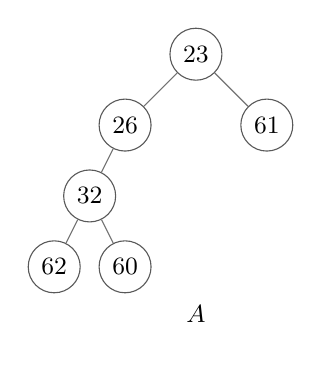
\begin{tikzpicture}[ltq]
\node {23}
    child {node {26} child {node {32} child {node {62}} child {node {60}}} child[missing]}
    child {node {61}};
\node[draw=none, font=\small] at (0,-3.3) {$A$};
\end{tikzpicture}\hspace{1.5cm}%
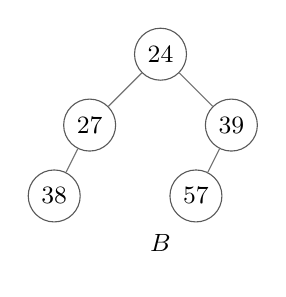
\begin{tikzpicture}[ltq]
\node {24}
    child {node {27} child {node {38}} child[missing]}
    child {node {39} child {node {57}} child[missing]};
\node[draw=none, font=\small] at (0,-2.4) {$B$};
\end{tikzpicture}
\end{center}

\item\label{hp-q-wblt} （證明）\textbf{重量左傾樹}：令 $w(x)$ 是以 $x$ 為根的子樹的節點數（$w(\NIL) = 0$），
規定每個節點都有 $w(x.\mathit{left}) \ge w(x.\mathit{right})$。 證明從根一路往右走到 \NIL，
經過的節點數不超過 $\lg(n + 1)$。

\item （計算、追蹤）二項堆積。
\begin{enumerate}
\item $n = 13$ 的二項堆積有幾棵樹？ 各是哪一階？
\item $B_5$ 有幾個節點在深度 $2$？
\item 把 $36, 14, 52, 29, 8, 61, 23, 47, 17, 40$ 依序插入空的二項堆積，寫出最後的各棵樹，
以及總共連結了幾次。
\item 接著取出最小值，寫出結果。
\end{enumerate}

\item （選擇，可能不只一個答案；計算）
\begin{enumerate}
\item 下列關於費氏堆積的敘述，哪些正確？ (A) \proc{Extract-Min} 最壞情況是 $O(\lg n)$。
(B) 從空的堆積插入 $n$ 個元素，接著的第一次 \proc{Extract-Min} 實際成本是 $\Theta(n)$。
(C) 某一次 \proc{Decrease-Key} 的實際成本可能超過常數。 (D) 位能 $t(H) + 2m(H)$ 在任何
時候都不小於 $0$。
\item Dijkstra 演算法在 $n$ 個點、$m$ 條邊的圖上做 $n$ 次 \proc{Insert}、$n$ 次
\proc{Extract-Min}、最多 $m$ 次 \proc{Decrease-Key}。 分別寫出用二元堆積和費氏堆積的總
時間；$m = \Theta(n^2)$ 時兩者各是多少？ $m = \Theta(n)$ 時呢？
\end{enumerate}
\end{enumerate}

\section{歷屆試題}
\label{sec:hp-pastexam}

以下是研究所入學考試的原題，題目照原卷（語言、記號、配分照錄）。 詳解在本章最後。

\begin{pastexam}[label={px:hp-1}]{中正資工所甲組 114 學年度 第 3 題}
(5\%) (Choose \underline{one} best answer) Consider the integer array \{52, 21, 40, 33, 88, 57, 46, 71\}. What will the array look like after heapifying it to a Max Heap? Note that we use the bottom-up method that runs in $O(n)$ time.
\begin{enumerate}[label=(\alph*)]
\item \{88, 71, 57, 52, 21, 40, 46, 33\}
\item \{88, 71, 57, 52, 46, 40, 33, 21\}
\item \{21, 33, 40, 46, 52, 57, 71, 88\}
\item \{88, 71, 57, 52, 33, 40, 46, 21\}
\item None of the above.
\end{enumerate}
\end{pastexam}

\begin{pastexam}[label={px:hp-2}]{臺科大資工所 110 學年度 第 6 題（節錄 (d)(e) 小題）}
Answer the following questions. (28\%)
\begin{enumerate}[label=(\alph*), start=4]
\item Draw the binary min heap that results from inserting 12, 9, 14, 16, 4, 17, 6, 8, 2 in that order into an initially empty binary heap. Draw the final tree. (10\%)
\item Remove the first two smallest values from the heap created in (d) and reconstruct the min heap. Draw the resulting tree. (5\%)
\end{enumerate}
\end{pastexam}

\begin{pastexam}[label={px:hp-3}]{成大資訊聯招 113 學年度 第 2 題}
\textbf{[1\%, 1\%, 3\%]} Considering the data pairs with keys in the given order: 20, 5, 10, 18, 4, 22, 11, 32, 21, as inputs to create a tree.
\begin{enumerate}[label=\roman*)]
\item If you create a \underline{max heap} for them, what is the level of the node containing 5?
\begin{enumerate}[label=(\Alph*)]
\item 1
\item 2
\item 3
\item 4
\item None of the above
\end{enumerate}
\item If you create a \underline{min heap} for them, which of the following statements is true?
\begin{enumerate}[label=(\Alph*)]
\item The node containing 11 is in the left subtree of the root.
\item The node containing 18 is in the right subtree of the root.
\item The node containing 20 is the root.
\item The node containing 21 is at level 3.
\item None of the above.
\end{enumerate}
\item If you create a \underline{symmetric min-max heap} for them, which of the following statements is true?
\begin{enumerate}[label=(\Alph*)]
\item To delete the node containing 5, the node containing 21 is used to replace the deleted node.
\item There are two nodes at level 4.
\item The leftmost grandchild of the root is 5.
\item The keys of the nodes in the right subtree of the root are 32, 10, and 20.
\item None of the above.
\end{enumerate}
\end{enumerate}
\end{pastexam}

\begin{pastexam}[label={px:hp-4}]{臺大資工所 113 學年度 第 2 題}
（原卷說明：本題為複選題。）

(5 points) A Maximum Binary Tree (abbreviated as MaxBT) is defined as a binary tree that adheres to the max-heap property without the necessity of following the complete binary tree property. In a MaxBT, each node $p$ consists of a value ($p$.data) and two links ($p$.left and $p$.right) pointing to the left and right children, respectively. A link to nil indicates the absence of further children.

The provided pseudocode, although incomplete, implements a recursive function for merging two MaxBTs into a single MaxBT. This function takes the root nodes of the two MaxBTs (\emph{root1} and \emph{root2}) as input and returns the root node of the merged MaxBT.
\begin{center}
\small
\begin{tabular}{rl}
1: & function MergeMaxBinaryTrees(\emph{root1}, \emph{root2}) \\
2: & \quad if \emph{root1} = nil then return \underline{\makebox[1.6cm]{(a)}} end if \\
3: & \quad if \emph{root2} = nil then return \underline{\makebox[1.6cm]{(b)}} end if \\
4: & \quad if \emph{root1}.data $>$ \emph{root2}.data then \\
5: & \quad\quad \underline{\makebox[1.6cm]{(c)}} $\leftarrow$ MergeMaxBinaryTrees(\underline{\makebox[1.6cm]{(d)}}, \underline{\makebox[1.6cm]{(e)}}) \\
6: & \quad\quad return \underline{\makebox[1.6cm]{(f)}} \\
7: & \quad else \\
8: & \quad\quad \underline{\makebox[1.6cm]{(g)}} $\leftarrow$ MergeMaxBinaryTrees(\underline{\makebox[1.6cm]{(h)}}, \underline{\makebox[1.6cm]{(i)}}) \\
9: & \quad\quad return \underline{\makebox[1.6cm]{(j)}} \\
10: & \quad end if \\
11: & end function
\end{tabular}
\end{center}
Assuming all the blanks in the above function have been appropriately filled to ensure its proper functioning, please select the correct description(s) below.
\begin{enumerate}[label=\Alph*.]
\item (b) and (f) are the same.
\item (c), (d), and (e) are all distinct.
\item In the cases of (c) and (g), each has only one correct answer.
\item Exchanging the filled content of (h) and (i) leads to a correct implementation.
\item The function works correctly even when the two arguments passed into it refer to the same tree.
\end{enumerate}
\end{pastexam}

\begin{pastexam}[label={px:hp-5}]{成大電通所 110 學年度 第 2 題（節錄 (b)(c) 小題）}
(\textbf{20 pts}) Heap
\begin{enumerate}[label=\alph*., start=2]
\item (4 \textbf{pts}) Describe the properties of a binomial min heap (i.e., four conditions).
\item (4 \textbf{pts}) Please show the resulting figure after you delete the node 1 in the following binomial min heap

\begin{center}
\begin{tikzpicture}[x=0.9cm,y=-0.9cm,
  v/.style={circle,draw,thick,inner sep=0pt,minimum size=6mm,font=\small},
  a/.style={-{Latex[length=2.2mm]},thick}]
\node[anchor=east] (hd) at (2.9,0.35) {Head[H]};
\node[v] (r14) at (4.3,0.35) {14};
\node[v] (r1) at (6.65,0.35) {1};
\node[v] (r6) at (11.75,0.35) {6};
\node[v] (a10) at (5.3,1.35) {10};
\node[v] (a23) at (6.65,1.35) {23};
\node[v] (a20) at (5.3,2.45) {20};
\node[v] (b10) at (9.5,1.35) {10};
\node[v] (b7) at (10.6,1.35) {7};
\node[v] (b15) at (11.75,1.35) {15};
\node[v] (b13) at (8.4,2.45) {13};
\node[v] (b12) at (9.5,2.45) {12};
\node[v] (b19) at (10.6,2.45) {19};
\node[v] (b30) at (8.4,3.45) {30};
\draw[a] (hd) -- (r14);
\draw[a] (r14) -- (r1);
\draw[a] (r1) -- (r6);
\draw[a] (r1) -- (a10);
\draw[a] (r1) -- (a23);
\draw[a] (a10) -- (a20);
\draw[a] (r6) -- (b10);
\draw[a] (r6) -- (b7);
\draw[a] (r6) -- (b15);
\draw[a] (b10) -- (b13);
\draw[a] (b10) -- (b12);
\draw[a] (b7) -- (b19);
\draw[a] (b13) -- (b30);
\end{tikzpicture}
\end{center}
\end{enumerate}
\end{pastexam}

\section{實作練習}
\label{sec:hp-practice}

下面是 Aki-Judge 上和本章相關的題目。 前幾題只要交標頭檔和函式，不寫 \texttt{main}；交
之前先用本章的範例和觀念題的資料自己測一次，特別是空的堆積、只有一個元素、所有元素相
等的情況。

\begin{center}
\begin{tabular}{llc}
\toprule
小節 & 題目 & 難度 \\
\midrule
二元堆積 & \akiref{check-min-heap}{檢查陣列是否為最小堆積} & 暖身 \\
二元堆積 & \akiref{min-heap-operations}{最小堆積的基本操作} & 基本 \\
由下而上建堆積 & \akiref{bottom-up-max-heap}{由下而上建立最大堆積} & 基本 \\
由下而上建堆積 & \akiref{heapsort-an-array}{以堆積排序整數陣列} & 基本 \\
優先佇列 & \akiref{kth-largest-element}{第 K 大的元素} & 基本 \\
優先佇列 & \akiref{merge-sorted-lists}{合併多個已排序數列} & 基本 \\
優先佇列 & \akiref{priority-queue-with-decrease}{可降低數值的優先佇列} & 進階 \\
優先佇列 & \akiref{halving-string-queue}{對半拆字串佇列} & 進階 \\
$d$ 元堆積 & \akiref{ternary-min-heap-with-replace}{三叉最小堆積與替換操作} & 進階 \\
\bottomrule
\end{tabular}
\end{center}

幾題的提示：

\begin{itemize}
\item 「由下而上建立最大堆積」的題目把這個方法叫做 Floyd 的方法（R. W. Floyd 在 1964 年
提出），就是第~\ref{sec:hp-build}~節的 \proc{Build-Max-Heap}，C 從 \texttt{n / 2 - 1} 倒
著做到 \texttt{0}。
\item 「以堆積排序整數陣列」先讀第~\ref{sec:hp-build}~節最後一小段，完整的虛擬碼和分析在第~\ref{sec:so-heap}~節。 常見的錯是每次把根
換到尾端以後，下沉時仍然用原本的大小 $n$，把已經排好的尾端又拉回堆積。
\item 「第 K 大的元素」和「合併多個已排序數列」照第~\ref{sec:hp-pq}~節「其他常見用法」的
做法，時間分別是 $O(n \lg k)$ 和 $O(N \lg k)$。
\item 「可降低數值的優先佇列」就是範例~\ref{ex:hp-er-queue} 的帶索引堆積：開一個位置陣
列，每次交換都更新。
\item 「對半拆字串佇列」每次取出字典序最小的片段再切成兩半放回去。 片段不必複製字串，記
住它在原字串的起點和長度就好，比較時用 \texttt{memcmp} 比共同的長度，再比長度。
\item 「三叉最小堆積與替換操作」照第~\ref{sec:hp-dary}~節的公式；題目規定幾個子節點一樣
小時取位置最小的，\texttt{R x} 就是第~\ref{sec:hp-pq}~節說的 replace，只做一次下沉，和
「先取出再插入」得到的陣列不一樣。
\end{itemize}

\section{讀完你應該會}
\label{sec:hp-checklist}

\begin{itemize}
\item 給一串數，畫出依序插入二元堆積（最大或最小）的每一步，以及取出最大（最小）值時下
沉的每一步，樹和陣列都會寫；從 $0$ 或從 $1$ 編號的位置公式都能正確使用。
\item 用由下而上的方法建堆積，寫出逐步陣列，並證明它的時間是 $\Theta(n)$。
\item 寫出帶索引的堆積，說明 decrease-key 和刪除任意元素為什麼需要位置陣列、刪除時為什麼
上浮和下沉都要試；知道相同的鍵要靠加入順序來分先後。
\item 寫出 $d$ 元堆積的位置公式和高度，說明 $d$ 變大時哪些操作變快、哪些變慢。
\item 在最小最大堆積、deap、對稱最小最大堆積上做插入、取出最小值和最大值，每一步都畫得出
來；寫出 deap 的對應點公式，說出 SMMH 的 P1--P3，知道區間堆積和 SMMH 的關係。
\item 合併兩棵左傾樹並更新 $s$；在二項堆積上做插入（含進位）、合併和取出最小值，每一步都
畫得出來。
\item 說出費氏堆積各操作的平攤成本，用位能 $t(H) + 2m(H)$ 說明插入、取出最小值、減少鍵
值的平攤成本從哪裡來，並分清楚平攤和最壞。
\end{itemize}

\textbf{延伸閱讀}（書末會整理完整的參考資料）

\begin{itemize}
\item Thomas H. Cormen 等，\textit{Introduction to Algorithms}，第 4 版，第 6 章：二元
堆積、建堆積的線性時間分析、堆積排序和優先佇列，章末問題有 $d$ 元堆積。 費氏堆積在第
4 版只在第五部的導言提到結論，完整的內容和分析在第 3 版第 19 章；第 2 版第 19 章是二項
堆積。
\item Ellis Horowitz、Sartaj Sahni、Susan Anderson-Freed，\textit{Fundamentals of Data
Structures in C}，第 9 章：最小最大堆積、左傾樹、二項堆積、費氏堆積都有 C 程式，各版的
節次稍有不同；二項堆積用的是延遲合併的版本。
\item Sartaj Sahni，``Double-Ended Priority Queues''，收在 Dinesh P. Mehta、Sartaj Sahni 編，
\textit{Handbook of Data Structures and Applications}（Chapman \& Hall/CRC，2005）第 8 章：
對稱最小最大堆積、區間堆積、最小最大堆積和 deap 放在一起比較。 deap 最早見於 Svante
Carlsson，``The Deap---A Double-Ended Heap to Implement Double-Ended Priority Queues''，
\textit{Information Processing Letters} 26 (1987)；SMMH 見於 A. Arvind、C. Pandu Rangan，
``Symmetric Min-Max Heap: A Simpler Data Structure for Double-Ended Priority Queue''，
\textit{Information Processing Letters} 69 (1999)。
\item Mark Allen Weiss，\textit{Data Structures and Algorithm Analysis in C}，第 6 章：
$d$ 元堆積、左傾堆積（用 npl 的定義）、斜堆積和二項佇列，取向偏實作。
\item 《C 程式設計基礎》第~19~章：用指標和 \texttt{malloc} 建二元樹的基本功，寫左傾樹前
可以先複習。
\end{itemize}

\addcontentsline{toc}{section}{觀念題解答}
\section*{觀念題解答}

\begin{enumerate}
\item (a)、(c)、(e)。 (a)：$90 \ge 70, 80$；$70 \ge 20, 60$；$80 \ge 75, 10$。 (b)：$A[6] =
85$ 比父節點 $A[3] = 70$ 大。 (c)：相等是允許的。 (d)：$A[4] = 40$ 比父節點 $A[2] = 30$
大。 (e)：$i > \lfloor i/2 \rfloor$，排在後面的不比前面的大。

\item 每列是操作之後的陣列，括號是交換次數。
\begin{center}
\begin{tabular}{lcl}
\toprule
操作 & 交換 & 陣列 \\
\midrule
插入 24 & 0 & 24 \\
插入 11 & 1 & 11 24 \\
插入 39 & 0 & 11 24 39 \\
插入 7 & 2 & 7 11 39 24 \\
插入 52 & 0 & 7 11 39 24 52 \\
插入 30 & 1 & 7 11 30 24 52 39 \\
插入 18 & 1 & 7 11 18 24 52 39 30 \\
插入 45 & 0 & 7 11 18 24 52 39 30 45 \\
取出 7 & 2 & 11 24 18 45 52 39 30 \\
取出 11 & 1 & 18 24 30 45 52 39 \\
\bottomrule
\end{tabular}
\end{center}
取出 $7$：$45$ 搬到根，和較小的子節點 $11$ 交換，再和 $24$ 交換。 取出 $11$：$30$ 搬到
根，和 $18$ 交換，到了位置 $3$，子節點 $39$ 比它大，停。

\item
\begin{enumerate}
\item $n = 9$，$i$ 從 $4$ 做到 $1$。
\begin{center}
\begin{tabular}{lcl}
\toprule
& 交換 & 陣列 \\
\midrule
$i = 4$ & 1 & 33 18 56 48 41 27 62 15 9 \\
$i = 3$ & 1 & 33 18 62 48 41 27 56 15 9 \\
$i = 2$ & 1 & 33 48 62 18 41 27 56 15 9 \\
$i = 1$ & 2 & 62 48 56 18 41 27 33 15 9 \\
\bottomrule
\end{tabular}
\end{center}
共交換 $5$ 次。 $i = 2$ 時 $18$ 和較大的子節點 $48$ 交換後，到了位置 $4$，子節點 $15$、
$9$ 都比它小，停。
\item 依序插入的結果是 $\langle 62, 48, 56, 41, 18, 27, 33, 9, 15 \rangle$，和 (a) 不同。
\end{enumerate}

\item
\begin{enumerate}
\item 深度 $d$ 的節點有 $d$ 個祖先，由堆積性質，它們都比這個節點大（元素互不相同）。
如果這個節點是第 $k$ 大，比它大的只有 $k - 1$ 個，所以 $d \le k - 1$。
\item 第 $2$ 大的深度不超過 $1$，又不是根（根是第 $1$ 大），所以在深度 $1$，也就是位置
$2$ 或 $3$。
\item 如果最小的元素有子節點，子節點比它小，矛盾，所以它是葉節點，在位置
$\lfloor n/2 \rfloor + 1$ 到 $n$ 之間。 每個葉節點都有可能：由大到小排好的陣列是最大堆積，
最小值在位置 $n$；把它和任何一個葉節點位置 $\ell$ 的數對調，位置 $\ell$ 沒有子節點，位置
$n$ 的父節點 $\lfloor n/2 \rfloor < \ell$ 比換過去的數大，仍是合法的堆積。
\end{enumerate}

\item 不變量：第 3 行的迴圈每一輪開始時，位置 $i + 1, \ldots, n$ 的每個節點都是一個最大
堆積的根。

初始：$i = \lfloor n/2 \rfloor$，位置 $\lfloor n/2 \rfloor + 1$ 到 $n$ 都是葉節點，一個節點
是最大堆積。

維持：$i$ 的子節點 $2i$、$2i + 1$ 都大於 $i$，由不變量它們都是最大堆積的根（不存在就不
用管），所以 \proc{Sift-Down}$(A, i)$ 之後以 $i$ 為根的子樹是最大堆積，裡面每個節點也都是
最大堆積的根。 \proc{Sift-Down} 只改動這棵子樹裡的位置，其他位置的子樹沒有被動到。 所以位
置 $i, i + 1, \ldots, n$ 都是最大堆積的根；下一輪 $i$ 減 $1$，不變量成立。

結束：迴圈在 $i = 0$ 停下，位置 $1, \ldots, n$ 都是最大堆積的根，特別是位置 $1$，也就是
整個陣列是最大堆積。

\item
\begin{enumerate}
\item $\lfloor \lg i \rfloor$ 在 $i = 1$ 到 $10$ 是 $0, 1, 1, 2, 2, 2, 2, 3, 3, 3$，和是
$19$。
\item 上界：每一項不超過 $\lg n$，$S(n) \le n \lg n$。 下界：$i \ge n/2$ 的項有至少
$n/2$ 項，每一項 $\lfloor \lg i \rfloor \ge \lg(n/2) - 1 = \lg n - 2$，所以
$S(n) \ge \frac{n}{2}(\lg n - 2)$，$n \ge 16$ 時至少 $\frac{n}{4}\lg n$。 所以
$S(n) = \Theta(n \lg n)$。
\end{enumerate}

\item (a)、(c)、(d)。 (b)：最大值在某個葉節點，要看 $\lceil n/2 \rceil$ 個葉節點，
$\Theta(n)$。 (c)：堆積只保證父子的大小，不能像二元搜尋那樣排除一半。 (d)：把兩個陣列接
起來，用 \proc{Build-Max-Heap}（或最小堆積版）建一次，$O(n)$。 (e)：同一層之間沒有任何
規定。

\item
\begin{enumerate}
\item 父節點 $\lfloor (100 - 2)/4 \rfloor + 1 = 25$。 位置 $25$ 的子節點是
$4 \cdot 24 + 2 = 98$ 到 $4 \cdot 25 + 1 = 101$，也就是 $98, 99, 100, 101$。
\item $h = \lceil \log_4(3 \cdot 1000 + 1) \rceil = \lceil \log_4 3001 \rceil = 6$
（$4^5 = 1024 < 3001 \le 4096 = 4^6$）。 驗算：高度 $5$ 最多 $(4^5 - 1)/3 = 341$ 個節點，
高度 $6$ 最多 $(4^6 - 1)/3 = 1365$ 個，$341 < 1000 \le 1365$。
\item 每往下一層，在最多 $d$ 個子節點裡找最小的要比 $d - 1$ 次，再和自己比 $1$ 次，共
$d$ 次。 從根（深度 $0$）往下最多走到深度 $h - 1$，也就是 $h - 1$ 層，所以最多
$d(h - 1)$ 次。
\item $n \approx 10^3$。 上浮和下沉最多走「高度減 $1$」層。 $d = 2$：高度
$\lfloor \lg 1000 \rfloor + 1 = 10$，最多走 $9$ 層，decrease-key 共
$10^6 \times 9 = 9 \times 10^6$，取出共 $10^3 \times 2 \times 9 \approx 1.8 \times 10^4$。
$d = 32$：高度 $\lceil \log_{32} 31001 \rceil = 3$（$32^2 = 1024 < 31001 \le 32^3$），最多
走 $2$ 層，decrease-key 共 $2 \times 10^6$，取出共
$10^3 \times 32 \times 2 = 6.4 \times 10^4$。 總數 $d = 32$ 大約是 $2.1 \times 10^6$，
比 $d = 2$ 的大約 $9 \times 10^6$ 少很多，選 $d = 32$。 decrease-key 遠多於取出時，$d$ 要取大。
\end{enumerate}

\item
\begin{enumerate}
\item 深度 $0$（最小層）：$10$；深度 $1$（最大層）：$65, 70$；深度 $2$（最小層）：$20,
40, 30, 60$；深度 $3$（最大層）：$25, 45, 50$。 檢查：$10$ 不大於所有元素；$65$ 不小於
$20, 40, 25, 45, 50$；$70$ 不小於 $30, 60$；$20$ 不大於 $25, 45$；$40$ 不大於 $50$。
\item $15$ 放在位置 $11$（最大層），父節點 $A[5] = 40$ 在最小層，$15 < 40$，$40$ 挪到位置
$11$；從位置 $5$ 沿最小層往上，祖父 $A[1] = 10$ 不比 $15$ 大，停。 陣列
$\langle 10, 65, 70, 20, 15, 30, 60, 25, 45, 50, 40 \rangle$。
\item 最大值是 $A[2]$、$A[3]$ 中較大的 $70$。 拿出最後一個 $x = 40$，從位置 $3$ 開始：子
節點 $30, 60$（沒有孫節點）中最大的是 $A[7] = 60$，是子節點，$60$ 搬到位置 $3$，$40$ 放
進位置 $7$。 陣列 $\langle 10, 65, 60, 20, 15, 30, 40, 25, 45, 50 \rangle$。
\item 取出 $10$，拿出 $x = 50$。 根的子節點 $65, 60$、孫節點 $20, 15, 30, 40$ 中最小的是
$A[5] = 15$（孫節點），搬到根；它的父節點 $A[2] = 65$ 不比 $50$ 小，不用對調。 位置 $5$
沒有子節點了（$n = 9$），$50$ 放進位置 $5$。 陣列
$\langle 15, 65, 60, 20, 50, 30, 40, 25, 45 \rangle$。
\end{enumerate}

\item
\begin{enumerate}
\item 位置 $2$ 到 $10$ 依序是 $13,\allowbreak 68,\allowbreak 27,\allowbreak 16,\allowbreak 61,\allowbreak 44,\allowbreak 40,\allowbreak 28,\allowbreak 34$；最小堆積的根 $13$ 有子節點 $27$、$16$，$27$ 的子節點是 $40$、$28$，$16$ 的子節點是 $34$；
最大堆積的根 $68$ 有子節點 $61$、$44$。 位置 $4$、$5$ 在深度 $2$，對應點是 $4 + 2 = 6$、
$5 + 2 = 7$；位置 $8, 9, 10$ 在深度 $3$，對應點 $12, 13, 14$ 都超過 $10$，改用父節點 $6, 6, 7$。
檢查：$27 \le 61$、$16 \le 44$、$40 \le 61$、$28 \le 61$、$34 \le 44$，兩邊各自也是堆積，所以是
deap。
\item 插入 $94$：放在位置 $11$（最小堆積），對應點 $15$ 改用 $7$；$94 > A[7] = 44$，$44$ 搬到位
置 $11$，$94$ 從位置 $7$ 上浮，比 $A[3] = 68$ 大，$68$ 挪到位置 $7$，$94$ 到位置 $3$：
$\langle 13, 94, 27, 16, 61, 68, 40, 28, 34, 44 \rangle$。 插入 $21$：放在位置 $12$（最大堆積），
對應點 $12 - 4 = 8$ 沒有子節點；$21 < A[8] = 40$，$40$ 搬到位置 $12$，$21$ 從位置 $8$ 上浮，
比 $A[4] = 27$ 小，$27$ 挪到位置 $8$，再和 $A[2] = 13$ 比，停在位置 $4$：
$\langle 13, 94, 21, 16, 61, 68, 27, 28, 34, 44, 40 \rangle$。
\item 取出 $94$，最後一格的 $40$ 拿出來。 洞從位置 $3$ 往下，子節點 $61, 68$ 中較大的 $68$ 上
來，洞到位置 $7$，沒有子節點（$14 > 11$）。 對應點 $7 - 2 = 5$ 有子節點 $34, 44$，取較大的
$44$（位置 $11$）；$40 < 44$，$44$ 搬到位置 $7$，$40$ 從位置 $11$ 上浮，父節點 $A[5] = 16$ 比它
小，停：$\langle 13, 68, 21, 16, 61, 44, 27, 28, 34, 40 \rangle$。 只和 $A[5] = 16$ 比的話，
$40$ 會留在位置 $7$，得到 $\langle 13, 68, 21, 16, 61, 40, 27, 28, 34, 44 \rangle$；位置 $11$ 的
$44$ 對應點 $15$ 超出範圍，改用 $7$，$44 > 40$，違反定義的第 2 條。
\item 取出 $13$，最後一格的 $40$ 拿出來。 洞從位置 $2$ 往下：$21, 16$ 中 $16$ 上來，洞到位置
$5$；它只剩子節點 $34$，$34$ 上來，洞到位置 $10$。 對應點 $14$ 改用 $7$；$40 \le A[7] = 44$，留
在最小堆積，父節點 $34$ 比它小，停：$\langle 16, 68, 21, 34, 61, 44, 27, 28, 40 \rangle$。
\end{enumerate}

\item
\begin{enumerate}
\item (A)、(C) 是。 (B) 位置 $6$、$7$ 是兄弟，$30 > 20$，違反 P1。 (D) 位置 $10$ 的祖父是 $2$，
$45 > A[5] = 40$，違反 P3（雖然 $45 \le A[3] = 50$）。
\item 每列是插入後的 $A[2..]$。
\begin{center}
\begin{tabular}{ll}
\toprule
插入 & 陣列 \\
\midrule
47 & 47 \\
18 & 18 47 \\
83 & 18 83 47 \\
60 & 18 83 47 60 \\
25 & 18 83 47 60 25 \\
91 & 18 91 47 60 25 83 \\
12 & 12 91 18 60 25 83 47 \\
70 & 12 91 18 70 25 83 47 60 \\
35 & 12 91 18 70 25 83 47 60 35 \\
\bottomrule
\end{tabular}
\end{center}
插入 $18$ 時位置 $3$ 是右子節點，比左兄弟 $47$ 小，對調。 插入 $83$、$91$ 時都比祖父（根）的右
子節點大，換上去。 插入 $12$：位置 $8$ 的祖父是 $2$，$12 < A[4] = 47$，$47$ 下來；再和根的左
子節點 $18$ 比，$18$ 下來，$12$ 到位置 $2$。 插入 $70$：位置 $9$ 比左兄弟 $47$ 大；祖父 $2$ 的右
子節點 $A[5] = 60 < 70$，$60$ 下來；再看根的兩個子節點 $12, 91$，停在位置 $5$。
\item 取出 $91$：最後的 $35$ 拿出來，洞在位置 $3$，候選 $A[5] = 70$、$A[7] = 83$，$83$ 上來，洞到
位置 $7$，左兄弟 $A[6] = 25$ 不比 $35$ 大，沒有子節點，$35$ 放進去：
$\langle 12, 83, 18, 70, 25, 35, 47, 60 \rangle$。 取出 $12$：最後的 $60$ 拿出來，洞在位置 $2$，
候選 $A[4] = 18$、$A[6] = 25$，$18$ 上來，洞到位置 $4$，右兄弟 $A[5] = 70$ 不比 $60$ 小；候選只
剩 $A[8] = 47$，$47 < 60$，上來，洞到位置 $8$，沒有兄弟也沒有子節點，$60$ 放進去：
$\langle 18, 83, 47, 70, 25, 35, 60 \rangle$。
\item 兄弟配對：$(2, 3)$、$(4, 5)$、$(6, 7)$、$(8, 9)$、$(10)$，得到根 $[12, 91]$，它的子節點
$[18, 70]$、$[25, 83]$，$[18, 70]$ 的子節點 $[47, 60]$ 和 $[35]$。 檢查：$[18, 70]$、$[25, 83]$
都在 $[12, 91]$ 裡；$[47, 60]$ 和 $35$ 都在 $[18, 70]$ 裡。
\end{enumerate}

\item 右邊路徑 $A$：$23, 61$；$B$：$24, 39$。 合成 $23 \to 24 \to 39 \to 61$。 由下往上：
$61$ 的 $s = 1$；$39$ 左邊 $57$（$s = 1$）、右邊 $61$（$s = 1$），不對調，$s = 2$；$24$
左邊 $27$（$s = 1$）小於右邊 $39$（$s = 2$），對調，$s = 2$；$23$ 左邊 $26$（$s = 1$）
小於右邊 $24$（$s = 2$），對調，$s = 2$。 結果用「根(左, 右)」寫成
\[
23\bigl(24(39(57, 61),\ 27(38, -)),\ 26(32(62, 60), -)\bigr),
\]
各節點的 $s$：$23{:}2$、$24{:}2$、$39{:}2$、$27{:}1$、$26{:}1$、$32{:}2$，葉節點都是 $1$。

取出 $23$：合併 $24(\ldots)$ 和 $26(\ldots)$。 右邊路徑 $24, 27$ 和 $26$ 合成
$24 \to 26 \to 27$。 $27$ 的 $s = 1$；$26$ 左邊 $32$（$s = 2$）不小於右邊 $27$（$s = 1$），
$s(26) = 2$；$24$ 左邊 $39$（$s = 2$）不小於右邊 $26$（$s = 2$），$s(24) = 3$。 結果
\[
24\bigl(39(57, 61),\ 26(32(62, 60),\ 27(38, -))\bigr).
\]

\item 對節點 $x$，令 $r(x)$ 是從 $x$ 一路往右走到 \NIL 經過的節點數，證明
$r(x) \le \lg(w(x) + 1)$。 對子樹大小歸納。 $x = \NIL$ 時兩邊都是 $0$。 否則
$w(x) = 1 + w(\mathit{left}) + w(\mathit{right})$，而 $w(\mathit{left}) \ge
w(\mathit{right})$，所以 $w(\mathit{right}) \le (w(x) - 1)/2$。 由歸納假設，
\[
r(x) = 1 + r(\mathit{right}) \le 1 + \lg\bigl(w(\mathit{right}) + 1\bigr)
\le 1 + \lg\frac{w(x) + 1}{2} = \lg\bigl(w(x) + 1\bigr).
\]
取 $x$ 是根，$w = n$，得證。 和定理~\ref{thm:hp-leftist} 一樣，合併只沿右邊路徑走，所以
重量左傾樹的合併也是 $O(\lg n)$。

\item
\begin{enumerate}
\item $13 = 1101_2$，三棵：$B_3$、$B_2$、$B_0$。
\item $\binom{5}{2} = 10$ 個。
\item 最後 $n = 10 = 1010_2$，兩棵：$B_1{:}\,17[40]$ 和
$B_3{:}\,8[14[29[52],\,36],\ 23[47],\ 61]$。 連結次數是 $10 - b(10) = 10 - 2 = 8$（逐次是
$0, 1, 0, 2, 0, 1, 0, 3, 0, 1$）。
\item 取出 $8$，子樹 $14[29[52], 36]$（$B_2$）、$23[47]$（$B_1$）、$61$（$B_0$）和剩下
的 $17[40]$（$B_1$）合併。 階數 $0$ 只有 $61$；階數 $1$ 有 $17[40]$、$23[47]$，連成
$17[23[47],\,40]$ 進位；階數 $2$ 有 $14[\ldots]$ 和進位，連成
$14[17[23[47],\,40],\ 29[52],\ 36]$。 結果 $n = 9 = 1001_2$：$B_0{:}\,61$ 和這棵 $B_3$。
\end{enumerate}

\item
\begin{enumerate}
\item (B)、(C)、(D)。 (A) 錯：$O(\lg n)$ 是平攤，(B) 就是一次 $\Theta(n)$ 的例子。 (C)：
連鎖剪下可能剪很多次。 (D)：棵數和標記數都不是負的。
\item 二元堆積：$O((n + m) \lg n)$。 費氏堆積：$n$ 次 \proc{Insert} 和 $m$ 次
\proc{Decrease-Key} 各 $O(1)$，$n$ 次 \proc{Extract-Min} 各 $O(\lg n)$，共
$O(m + n \lg n)$。 $m = \Theta(n^2)$：$O(n^2 \lg n)$ 對 $O(n^2)$，費氏堆積快一個
$\lg n$。 $m = \Theta(n)$：兩者都是 $O(n \lg n)$。
\end{enumerate}
\end{enumerate}

\addcontentsline{toc}{section}{歷屆試題詳解}
\section*{歷屆試題詳解}

\pastsol{px:hp-1}{中正資工所甲組 114 學年度 第 3 題}
答案是 (a)。 由下而上建堆積照虛擬碼~\ref{alg:hp-build}：$n = 8$，$i$ 從 $\lfloor 8/2 \rfloor = 4$
做到 $1$，每次對位置 $i$ 做 \proc{Sift-Down}。

\begin{center}
\begin{tabular}{lc*{8}{c}}
\toprule
& 交換 & 1 & 2 & 3 & 4 & 5 & 6 & 7 & 8 \\
\midrule
開始 & & 52 & 21 & 40 & 33 & 88 & 57 & 46 & 71 \\
$i = 4$ & 1 & 52 & 21 & 40 & 71 & 88 & 57 & 46 & 33 \\
$i = 3$ & 1 & 52 & 21 & 57 & 71 & 88 & 40 & 46 & 33 \\
$i = 2$ & 1 & 52 & 88 & 57 & 71 & 21 & 40 & 46 & 33 \\
$i = 1$ & 2 & 88 & 71 & 57 & 52 & 21 & 40 & 46 & 33 \\
\bottomrule
\end{tabular}
\end{center}

$i = 4$：$33$ 只有左子節點 $A[8] = 71$，交換。 $i = 3$：$40$ 和較大的子節點 $57$ 交換。 $i = 2$：
$21$ 和較大的子節點 $88$ 交換，到了位置 $5$，沒有子節點。 $i = 1$：$52$ 先和 $88$ 交換，到了位
置 $2$，子節點 $71, 21$ 中 $71$ 比它大，再交換，到了位置 $4$，子節點 $33$ 比它小，停。 結果
$\{88, 71, 57, 52, 21, 40, 46, 33\}$，就是 (a)。

其他選項：(b) 是由大到小排好的陣列，它也是最大堆積，但不是這個方法的結果。 (c) 是由小到大
排好，根是最小值，不是最大堆積。 (d) 也是合法的最大堆積（逐層檢查父子都成立），但位置 $5$
和 $8$ 的 $33$、$21$ 和由下而上的結果對調了。 (a) 正確，所以 (e) 不對。 題目問的是特定方法
的結果，「是不是合法的最大堆積」不夠，要真的做一次。

\pastsol{px:hp-2}{臺科大資工所 110 學年度 第 6 題（節錄 (d)(e) 小題）}
(d) 每次插入放在最後一格再上浮（第~\ref{sec:hp-trace}~節，最小堆積版）。 每列是插入之後的陣
列，位置從 $1$ 開始。

\begin{center}
\begin{tabular}{lc*{9}{c}}
\toprule
插入 & 交換 & 1 & 2 & 3 & 4 & 5 & 6 & 7 & 8 & 9 \\
\midrule
12 & 0 & 12 \\
9 & 1 & 9 & 12 \\
14 & 0 & 9 & 12 & 14 \\
16 & 0 & 9 & 12 & 14 & 16 \\
4 & 2 & 4 & 9 & 14 & 16 & 12 \\
17 & 0 & 4 & 9 & 14 & 16 & 12 & 17 \\
6 & 1 & 4 & 9 & 6 & 16 & 12 & 17 & 14 \\
8 & 2 & 4 & 8 & 6 & 9 & 12 & 17 & 14 & 16 \\
2 & 3 & 2 & 4 & 6 & 8 & 12 & 17 & 14 & 16 & 9 \\
\bottomrule
\end{tabular}
\end{center}

插入 $4$：放在位置 $5$，父節點 $A[2] = 12$ 比它大，交換；再和根 $9$ 交換。 插入 $8$：放在位置 $8$，
和父節點 $16$、再和 $9$ 交換，父節點 $4$ 比它小，停。 插入 $2$：位置 $9$ 往上的父節點依序是
$A[4] = 9$、$A[2] = 8$、$A[1] = 4$，都比它大，交換三次，$2$ 到根。 最後的樹是下圖 (a)。

(e) 取出 $2$：最後一格的 $9$ 搬到根，和較小的子節點 $4$ 交換，到了位置 $2$，子節點 $8, 12$ 中
$8$ 比它小，交換，到了位置 $4$，子節點只剩 $16$，停：
$\langle 4, 8, 6, 9, 12, 17, 14, 16 \rangle$。 取出 $4$：最後一格的 $16$ 搬到根，和較小的子節點
$6$ 交換，到了位置 $3$，子節點 $17, 14$ 中 $14$ 比它小，交換，到了位置 $7$，停：
$\langle 6, 8, 14, 9, 12, 17, 16 \rangle$，是下圖 (b)。

\begin{center}
\begin{tikzpicture}
\hpheap{0,0}{6.0}{2/n,4/n,6/n,8/n,12/n,17/n,14/n,16/n,9/n}{xa}
\hpheap{7.4,0}{4.6}{6/n,8/n,14/a,9/n,12/n,17/n,16/a}{xb}
\node[font=\small] at (0,-3.65) {(a) (d) 的答案};
\node[font=\small] at (7.4,-3.65) {(b) (e) 的答案};
\end{tikzpicture}
\end{center}

\pastsol{px:hp-3}{成大資訊聯招 113 學年度 第 2 題}
題目說 ``in the given order''，三小題都解讀成依序一個一個插入。 層數照題目的慣例（也是本書的
約定）從根算第 $1$ 層。 答案：i) (D)；ii) (E)；iii) (A)。

i) 依序插入最大堆積，每次之後的陣列：
\begin{center}
\small
\begin{tabular}{l*{9}{c}}
\toprule
插入 & 1 & 2 & 3 & 4 & 5 & 6 & 7 & 8 & 9 \\
\midrule
20 & 20 \\
5 & 20 & 5 \\
10 & 20 & 5 & 10 \\
18 & 20 & 18 & 10 & 5 \\
4 & 20 & 18 & 10 & 5 & 4 \\
22 & 22 & 18 & 20 & 5 & 4 & 10 \\
11 & 22 & 18 & 20 & 5 & 4 & 10 & 11 \\
32 & 32 & 22 & 20 & 18 & 4 & 10 & 11 & 5 \\
21 & 32 & 22 & 20 & 21 & 4 & 10 & 11 & 5 & 18 \\
\bottomrule
\end{tabular}
\end{center}
插入 $32$ 時它從位置 $8$ 一路換到根，把 $5$ 帶到位置 $8$。 位置 $8$ 的深度是
$\lfloor \lg 8 \rfloor = 3$，在第 $4$ 層，選 (D)。 （如果題目的層數從 $0$ 算，答案會變成 (C)；成大
的考卷沿用從 $1$ 算的定義。）

ii) 依序插入最小堆積：
\begin{center}
\small
\begin{tabular}{l*{9}{c}}
\toprule
插入 & 1 & 2 & 3 & 4 & 5 & 6 & 7 & 8 & 9 \\
\midrule
20 & 20 \\
5 & 5 & 20 \\
10 & 5 & 20 & 10 \\
18 & 5 & 18 & 10 & 20 \\
4 & 4 & 5 & 10 & 20 & 18 \\
22 & 4 & 5 & 10 & 20 & 18 & 22 \\
11 & 4 & 5 & 10 & 20 & 18 & 22 & 11 \\
32 & 4 & 5 & 10 & 20 & 18 & 22 & 11 & 32 \\
21 & 4 & 5 & 10 & 20 & 18 & 22 & 11 & 32 & 21 \\
\bottomrule
\end{tabular}
\end{center}
結果是 $\langle 4,\allowbreak 5,\allowbreak 10,\allowbreak 20,\allowbreak 18,\allowbreak 22,\allowbreak 11,\allowbreak 32,\allowbreak 21 \rangle$。 根的左子樹是位置 $2,\allowbreak 4,\allowbreak 5,\allowbreak 8,\allowbreak 9$，也就是 $5,\allowbreak 20,\allowbreak 18,\allowbreak 32,\allowbreak 21$；右子樹是位
置 $3, 6, 7$，也就是 $10, 22, 11$。 (A) $11$ 在右子樹，錯。 (B) $18$ 在左子樹，錯。 (C) 根是
$4$，錯。 (D) $21$ 在位置 $9$，第 $4$ 層，錯。 所以選 (E)。

iii) 照第~\ref{sec:hp-smmh}~節的 \proc{SMMH-Insert}，下表是每次之後的 $A[2..]$：
\begin{center}
\small
\begin{tabular}{l*{9}{c}}
\toprule
插入 & 2 & 3 & 4 & 5 & 6 & 7 & 8 & 9 & 10 \\
\midrule
20 & 20 \\
5 & 5 & 20 \\
10 & 5 & 20 & 10 \\
18 & 5 & 20 & 10 & 18 \\
4 & 4 & 20 & 10 & 18 & 5 \\
22 & 4 & 22 & 10 & 18 & 5 & 20 \\
11 & 4 & 22 & 10 & 18 & 5 & 20 & 11 \\
32 & 4 & 32 & 10 & 22 & 5 & 20 & 11 & 18 \\
21 & 4 & 32 & 10 & 22 & 5 & 20 & 11 & 18 & 21 \\
\bottomrule
\end{tabular}
\end{center}
插入 $5$：位置 $3$ 是右子節點，比左兄弟 $20$ 小，對調。 插入 $4$：位置 $6$ 的祖父是根，
$4 < A[2] = 5$，$5$ 下來。 插入 $22$：比 $A[3] = 20$ 大，$20$ 下來。 插入 $32$：位置 $9$ 的祖父是
$2$，$32 > A[5] = 18$，$18$ 下來；位置 $5$ 的祖父是根，$32 > A[3] = 22$，$22$ 下來，$32$ 到位置
$3$。 插入 $21$：位置 $10$ 的祖父是 $2$，$A[4] = 10 \le 21 \le A[5] = 22$，不動。 最後的樹如下
圖 (c)：空的根，第 $2$ 層 $4, 32$，第 $3$ 層 $10, 22, 5, 20$，第 $4$ 層 $11, 18, 21$。

(B) 第 $4$ 層有三個節點，錯。 (C) 根的孫節點由左到右是 $10, 22, 5, 20$，最左邊是 $10$，錯。
(D) 根的右子樹是位置 $3, 6, 7$，鍵是 $32, 5, 20$，不是 $32, 10, 20$，錯。 (A)：本書只定義了
取出最小值和最大值，題目沒有說刪除任意節點怎麼做；照取出最小值的做法類推，刪掉位置 $6$
的 $5$ 之後，拿最後一個節點的 $21$ 來補這個洞（洞沒有子節點；$21$ 比右兄弟 $A[7] = 20$ 大，
兩者再對調，最後是 $A[6] = 20$、$A[7] = 21$）。 「用 $21$ 那個節點來補」這件事成立，所以 (A)
對，選 (A)。 這也是唯一可能的答案：(B)、(C)、(D) 都確定是錯的。

\begin{center}
\begin{tikzpicture}
\hpheap{0,0}{5.6}{32/n,22/n,20/n,21/n,4/n,10/n,11/n,5/a,18/n}{ya}
\hpheap{6.6,0}{5.6}{4/n,5/n,10/n,20/n,18/n,22/n,11/n,32/n,21/n}{yb}
\node[font=\small] at (0,-3.65) {(a) 最大堆積，$5$ 在第 $4$ 層};
\node[font=\small] at (6.6,-3.65) {(b) 最小堆積};
\end{tikzpicture}

\begin{tikzpicture}
\hpheap{0,0}{6.0}{/e,4/n,32/n,10/n,22/n,5/a,20/n,11/n,18/n,21/n}{yc}
\node[font=\small] at (0,-3.65) {(c) 對稱最小最大堆積};
\end{tikzpicture}
\end{center}

\pastsol{px:hp-4}{臺大資工所 113 學年度 第 2 題}
答案是 A、D。 先把函式補完。 兩棵樹都不空時，根比較大的那個當新的根（$>$ 不成立時選
\emph{root2}，相等也可以），把它的某一棵子樹和另一整棵樹遞迴合併，結果接回同一邊。 這和
虛擬碼~\ref{alg:hp-meld} 左傾樹的 \proc{Meld} 是同一個架構，只是少了比較 $s$、對調左右那兩步。
一種正確的填法：

\begin{pseudo}[unbreakable]{臺大 113 第 2 題的一種填法}
\Function{MergeMaxBinaryTrees}{$\mathit{root1}, \mathit{root2}$}
    \If{$\mathit{root1} = \NIL$} \Return $\mathit{root2}$ \Comment{(a)} \EndIf
    \If{$\mathit{root2} = \NIL$} \Return $\mathit{root1}$ \Comment{(b)} \EndIf
    \If{$\mathit{root1}.\mathit{data} > \mathit{root2}.\mathit{data}$}
        \State $\mathit{root1}.\mathit{right} \gets$ \Call{MergeMaxBinaryTrees}{$\mathit{root1}.\mathit{right}, \mathit{root2}$} \Comment{(c)(d)(e)}
        \State \Return $\mathit{root1}$ \Comment{(f)}
    \Else
        \State $\mathit{root2}.\mathit{right} \gets$ \Call{MergeMaxBinaryTrees}{$\mathit{root1}, \mathit{root2}.\mathit{right}$} \Comment{(g)(h)(i)}
        \State \Return $\mathit{root2}$ \Comment{(j)}
    \EndIf
\EndFunction
\end{pseudo}

正確性對兩棵樹的節點總數歸納：遞迴呼叫的兩棵樹節點總數少了一個（新的根不在裡面），由歸納假
設回傳一棵 MaxBT，它的節點都來自原本的兩棵樹，所以都不大於新的根；接回去以後新的根仍然不小
於兩棵子樹的所有節點，整棵是 MaxBT。

逐個選項：
\begin{itemize}
\item[A.] 對。 (b) 是 \emph{root2} 為空時回傳 \emph{root1}；(f) 是 \emph{root1} 當新的根時回傳
\emph{root1}。 兩格都必須是 \emph{root1}。
\item[B.] 錯。 (c) 是被改寫的那個欄位，它原本指的子樹必須當作遞迴的一個參數傳進去，否則那棵子
樹就從樹上掉了。 所以 (c) 一定和 (d)、(e) 其中一個相同（例如上面的 (c) 和 (d) 都是
\emph{root1}.right）。
\item[C.] 錯。 MaxBT 不要求形狀，(c) 填 \emph{root1}.left（同時 (d) 或 (e) 改成
\emph{root1}.left）也一樣正確；(g) 同理。 每一格都至少有兩種正確答案。
\item[D.] 對。 上面的正確性論證沒有用到兩個參數的順序：交換 (h)、(i) 之後，遞迴呼叫仍然是合併同
樣兩棵樹，回傳的仍然是一棵包含它們全部節點的 MaxBT。 相等的情況也沒問題，相等時選誰當根都
滿足最大堆積性質。
\item[E.] 錯。 兩個參數是同一棵樹時，資料相等，走 else，把 \emph{root2}.right 改成「這棵樹和它
自己的右子樹合併」的結果，同一批節點被接到兩個地方。 最簡單的例子是只有一個節點 $r$：
\proc{MergeMaxBinaryTrees}$(r, r)$ 走 else，$r.\mathit{right} \gets$
\proc{MergeMaxBinaryTrees}$(r, \NIL) = r$，$r$ 的右子節點變成自己，不再是一棵樹。
\end{itemize}

補充：沒有像左傾樹那樣控制右邊路徑的長度，這個合併最壞要沿著很長的路徑遞迴，時間是
$\Theta(n)$，而左傾樹保證 $O(\lg n)$（定理~\ref{thm:hp-leftist}）。

\pastsol{px:hp-5}{成大電通所 110 學年度 第 2 題（節錄 (b)(c) 小題）}
(b) 照第~\ref{sec:hp-mergeable}~節的定義，二項最小堆積是一群樹，滿足：
\begin{enumerate}
\item 每棵樹都是二項樹 $B_k$（$B_0$ 是一個節點，$B_k$ 是兩棵 $B_{k-1}$ 把一棵的根接成另一棵根
的最左邊的子節點）。
\item 每棵樹都滿足最小堆積性質：每個節點的鍵不小於它的父節點。
\item 每個階數 $k$ 最多只有一棵 $B_k$；所以 $n$ 個元素時有哪幾棵樹由 $n$ 的二進位決定。
\item 各棵樹的根用根串列串起來，依階數由小到大排列（\texttt{Head[H]} 指向階數最小的那棵）。
\end{enumerate}

(c) 圖中的根串列是 $B_0{:}\,14$、$B_2{:}\,1[10[20],\,23]$、$B_3{:}\,6[10[13[30],\,12],\ 7[19],\
15]$，共 $13 = 1101_2$ 個元素。 照第~\ref{sec:hp-mergeable}~節的取出最小值：
\begin{enumerate}
\item 最小的根是 $1$，從根串列拿掉，剩下 $\{B_0{:}\,14,\ B_3{:}\,6[\ldots]\}$。
\item $1$ 的子樹由左到右是 $B_1{:}\,10[20]$、$B_0{:}\,23$，反過來排，成為另一個二項堆積：
$B_0{:}\,23$、$B_1{:}\,10[20]$。
\item 兩個堆積合併。 階數 $0$：$14$、$23$ 兩棵，連成 $14[23]$ 進位。 階數 $1$：$10[20]$ 和進位的
$14[23]$ 兩棵，根 $10 < 14$，$14$ 那棵掛到 $10$ 的最左邊，得到 $B_2{:}\,10[14[23],\,20]$ 進位。
階數 $2$：只有進位的那棵，留下。 階數 $3$：$6[\ldots]$，留下。
\end{enumerate}
結果有 $12 = 1100_2$ 個元素，兩棵樹：

\begin{center}
\begin{tikzpicture}[x=0.9cm,y=-0.9cm,
  v/.style={circle,draw,thick,inner sep=0pt,minimum size=6mm,font=\small},
  a/.style={-{Latex[length=2.2mm]},thick}]
\node[anchor=east] (hd) at (2.9,0.35) {Head[H]};
\node[v] (r10) at (4.6,0.35) {10};
\node[v] (c14) at (3.8,1.35) {14};
\node[v] (c20) at (5.4,1.35) {20};
\node[v] (c23) at (3.8,2.45) {23};
\node[v] (r6) at (9.9,0.35) {6};
\node[v] (b10) at (7.7,1.35) {10};
\node[v] (b7) at (8.8,1.35) {7};
\node[v] (b15) at (9.9,1.35) {15};
\node[v] (b13) at (6.6,2.45) {13};
\node[v] (b12) at (7.7,2.45) {12};
\node[v] (b19) at (8.8,2.45) {19};
\node[v] (b30) at (6.6,3.45) {30};
\draw[a] (hd) -- (r10);
\draw[a] (r10) -- (r6);
\draw[a] (r10) -- (c14);
\draw[a] (r10) -- (c20);
\draw[a] (c14) -- (c23);
\draw[a] (r6) -- (b10);
\draw[a] (r6) -- (b7);
\draw[a] (r6) -- (b15);
\draw[a] (b10) -- (b13);
\draw[a] (b10) -- (b12);
\draw[a] (b7) -- (b19);
\draw[a] (b13) -- (b30);
\end{tikzpicture}
\end{center}

也就是 $B_2{:}\,10[14[23],\,20]$ 和原本的 $B_3$。 圖中兩棵樹各有一個 $10$，鍵可以重複，不影響
做法。
